\documentclass[12pt,a4paper]{report}

\usepackage{dolgozat}

\usepackage{hyperref}

\usepackage{listings}
\usepackage{python}
\usepackage{cpp}

\linespread{1.2}

\begin{document}

% !TEX encoding = UTF-8 Unicode


\pagestyle{empty} %a címlapon ne legyen semmi=empty, azaz nincs fejléc és lábléc

\begin{flushleft}
\textsc{\bfseries Miskolci Egyetem}\\
Gépészmérnöki és Informatikai Kar\\
Analízis Intézeti Tanszék
\end{flushleft}

%A fõiskola logoja
{\large
\begin{center}
\vglue 1truecm
\textbf{\huge\textsc{Szakdolgozat}}\\
\vglue 1truecm

\epsfig{file=cimlap/ME_logo.eps, width=4.8truecm, height=4truecm}\\
\textbf{\textsc{Miskolci Egyetem}}
\end{center}}

\vglue 1.5truecm %függõleges helykihagyás

%A szakdolgozat címe, akár több sorban is
{\LARGE
\begin{center}
\textbf{Alternatív grafikus megjelenítési módok}
\end{center}}

\vspace*{2.5truecm}
%A hallgató neve, évfolyam, szak(ok), a konzulens(ek) neve
{\large
\begin{center}
\begin{tabular}{c}
\textbf{Készítette:}\\
Vécsi Ádám\\
Gazdasági informatikus BSc
\end{tabular}
\end{center}
\begin{center}
\begin{tabular}{c}
\textbf{Témavezetõ:}\\
Piller Imre, egyetemi tanársegéd
\end{tabular}
\end{center}}
\vfill
%Keltezés: Hely és év
{\large
\begin{center}
\textbf{\textsc{Miskolc, 2018}}
\end{center}}

\newpage

\cleardoublepage
\pagenumbering{gobble}
\tableofcontents
\cleardoublepage
\pagenumbering{arabic}

\newpage

\pagestyle{fancy}

% !TEX encoding = UTF-8 Unicode

\Chapter{Bevezetés}

A fényképek és videók készítése napjainkban már teljesen természetessé, megszokottá vált. Ennek köszönhetően népszerűvé váltak azok az eljárások és alkalmazások, melyek segítségével az eredeti felvételből valamilyen stilizált, művészi jellegű képet készíthetünk. Összefoglaló néven ezeket művészi szűrőknek nevezzük.

A dolgozat célja, hogy bemutassa ezen szűrők matematikai hátterét, megvalósítási módját, illetve saját készítésű szűrőket is felvonultasson.

Fiatalok körében eléggé elterjedtek a kép feldolgozással kapcsolatos alkalmazások, gondoljunk csak bele, hogy a napijainkban használatos közösségi alkalmazások mindegyikében megtalálható ez az opció. Akár arc felismeréssel képeken, valós időben és mozgóképeken, vagy akár előre kidolgozott szűrők segítségével, amik elmossák a szineket, kiemelik az éleket vagy valamilyen módon átalakítják a képeket. Ezekre is ki fogok térni a dolgozat során.
% népszerű alkalmazások

Részletezni szeretném a különböző képfeldolgozási műveletek matematikai hátterét is. Láthatók lesznek, a matematikai leírásoknál példák is, valamint ábrák.
% matematikai háttér

Saját készítésű szűrőim rajzfilm, ceruza rajz szerű, valamint festmény jellegűek. Szűrőket képekkel lépésről lépésre szeretném bemutatni, továbbá a C vagy C++ implementációját is részletezni fogom.
% saját algoritmusok

Mint említettem szűrőimet C vagy C++ programozási nyelven szeretném megírni, OpenCV könyvtár segítségével. Az OpenCV az egy ingyenes, képfeldolgozási algoritmusak tartalmazó könyvtár. A dolgozatom során, fogom részletezni magát a könyvtárat is.
% OpenCV

A végén szeretnék néhány tesztet is készíteni, azon szűrőkre amiket én fogok elkészíteni. A tesztek a szűrők feldolgozási idejére, valamint az egyes lépések feldolgozási idejére vonatkozik képek esetén. Tervben van az is, hogy a szűrőket megpróbálom megvalósítani úgy, hogy ne csak képek feldolgozására legyen alkalmas, hanem videón, esetleg valós időben is működjön. Ezek tesztelésére, egy képkocka per másodperc tesztet szeretnék alkalmazni, amivel kiderül, hogy egy másodperc alatt hány képkockát tudunk előállítani az egyes szűrők esetén.
% tesztek

A következő fejezeteben a művészi jellegű szűrőket szeretném prezentálni.

% !TEX encoding = UTF-8 Unicode

\Chapter{Művészi jellegű szűrők}

A mai világban elég népszerűek az olyan számítógépes vagy mobiltelefonos alkalmazások, amelyekkel fényképeket vagy videókat lehet átalakítani valós időben, képfeldolgozási módszerekkel. Dolgozatomban ezen alkalmazások működésének hátterével, jellemző algoritmusaival és megvalósítási módjukkal foglalkozom.

A művészi szűrők mögött komoly tudományos eredmények állnak. Többen foglalkoznak azzal, hogy egy-egy művészi jellegű hatás megvalósításának milyen lehetőségei vannak. Alapvetően nagyon irányzatként a témakörben az élek megtartásával történő szűrést \cite{artistic}, és a szegmentálásra épülő objektumkijelölést \cite{intellipaint} különíthetjük el.

A következő szakaszok egyelőre azt vizsgálják, hogy milyen területeken találkozhatunk a művészi szűrők alkalmazásával a népszerű weboldalak és alkalmazások körében.

\Section{Népszerű alkalmazási területek}

A fiatalok többsége ha képfeldolgozásról van szó egyből a közösségi média adta lehetőségekre gondol. Ilyen például az Instagram, Snapchat vagy a Messenger alkalmazások. Ezek az applikációk a telefonok, tabletek kameráját használja, mint a képek vagy videók forrását. Dolgozatomban ezek működésére is kitérek.

\SubSection{Közösségi alkalmazások}

A közösségi alkalmazásokba előszeretettel építenek különféle képfeldolgozási módszereket. \Aref{fig:social_media}. ábrán láthatunk egy-egy példát az Instagram, Snapchat és Messenger alkalmazások egy-egy szűrőjének alkalmazására. A következőkben ezen alkalmazások rövid áttekintésére kerül sor.

\paragraph{Instagram} 

Valószínűleg az Instagram egyik legismertebb applikáció, amely képekkel és képfeldolgozással foglalkozik \cite{instagram}. Ez az alkalmazás pontosan arra készült, hogy a felhasználók megoszthassák egymással  ezeket, majd különféle művészi szűrőkkel láthassanak el. A szűrők köre folyamatosan bővül, valamit egyre testreszabhatók lesznek, például lehet állítani a képek dőlésszögén, fényességén, hogy mennyire legyen kontrasztos, a színek melegségén, mennyire legyen elmosva és hogy hol legyenek az elmosódások.

\paragraph{Snapchat} 

A Snapchat is egy képfeldolgozással kapcsolatos alkalmazás \cite{snapchat}, bár teljesen más a koncepció mint az Instagram esetében. Itt is a barátainkkal, imerőseinkkel tudjuk megosztani a grafikus tartalmainkat, de ezek a nyilvánosság számára nem láthatók, csak azok láthatják akiknek adunk jogosultságot, hogy láthassák és ők is csak egy bizonyos ideig, amit mi határozunk meg küldéskor. Ez az alkalmazás nem csak egyszerűen művészi szűrőkkel foglalkozik, hanem képes detektálni az arcokat. Mivel az alkamazás felismeri az arcunkat, így különböző tárgyakat/effekteket képes rárakni ennek megfelelően, például napszemüveget, vicces sapkákat,  különböző fényeket, eltorzítja az arcunk vagy a szemünket.

\paragraph{Messenger} 

Ez az alkalmazás nem kifejezetten képfeldolgozással foglalkozik, azonban már megjelentek benne ezek a funkciók is. Ebben az alkalmazásban barátainkkal, imerőseinkkel tudunk chatelni, tartalmakat megosztani, akár privát módon, akár csoportosan \cite{messenger}. Képeinket hasonló módon tudjuk szerkeszteni, mint a Snapchat alkalmazással. Itt is arcfelismerés alapján tud rárakni az arcunkra a program mindenféle effektet. Ebben a programban elérhető a videóhívás is ahol szintén haszálhatók effektek.

\begin{figure}[ht]
\centering
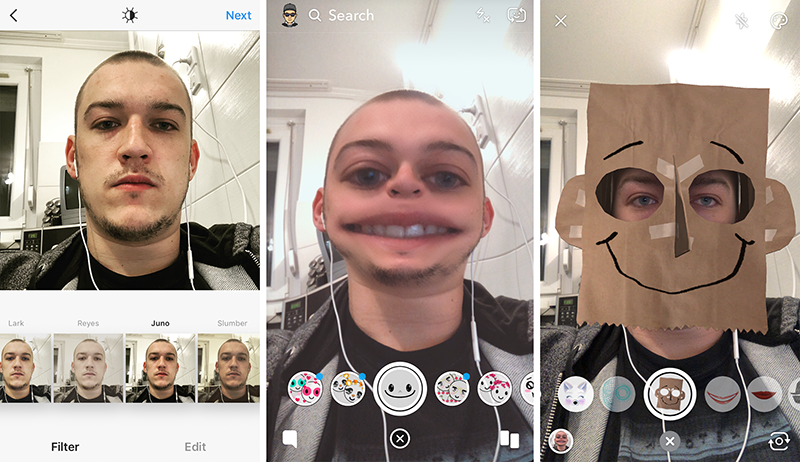
\epsfig{file=kepek/instasnapmess.png,scale=0.47}
\caption{Az Instagram, Snapchat és Messenger alkalmazások művészi szűrőiről készült képernyőfotók} 
\label{fig:social_media}
\end{figure}

\SubSection{Webkamera- és mobil alkalmazások}

A közösségi alkamazásokon kívül, van néhány olyan weboldal, mobil alkalmazás amely szintén komplikáltabb képfeldolgozási módszereket használ. A következőkben ezek közül a Prisma alkalmazást és a webkamerás alkalmazások néhány jellemzőjét mutatom be.

\paragraph{Prisma}

Ez az alkalmazás a képfeldolgozáshoz mesterséges intelligenciát, jellemzően neurális hálókat haszánál, hogy művészi szűrőkkel ellátott képeket hozzon létre \cite{prisma}. A felhasználó az alkalmazásba betölti az átalakítandó fényképet, kiválasztja a számára megfelelő szűrőt, pár másodperc múlva a szűrővel elláttott kép megjelenik az alkalmazásban. A képfeldolgozás a Prisma esetében távoli szerveren történik.

\paragraph{Webkamera alkalmazások} 

Számtalan olyan program, webalkalmazás van amely tartalmaz képfeldolgozási funkciókat. Egy ilyen például a \textit{Pixect} \cite{pixect}. Léteznek továbbá gyári beépített programok, amelyek a webkamera saját illesztőprogramjában találhatók meg, és különböző szűrőket tudnak rárakni a képekre. Művészi szűrőkkel ellátott képekre láthatunk néhány példát \aref{fig:prisma}. ábrán.

\begin{figure}[ht]
\centering
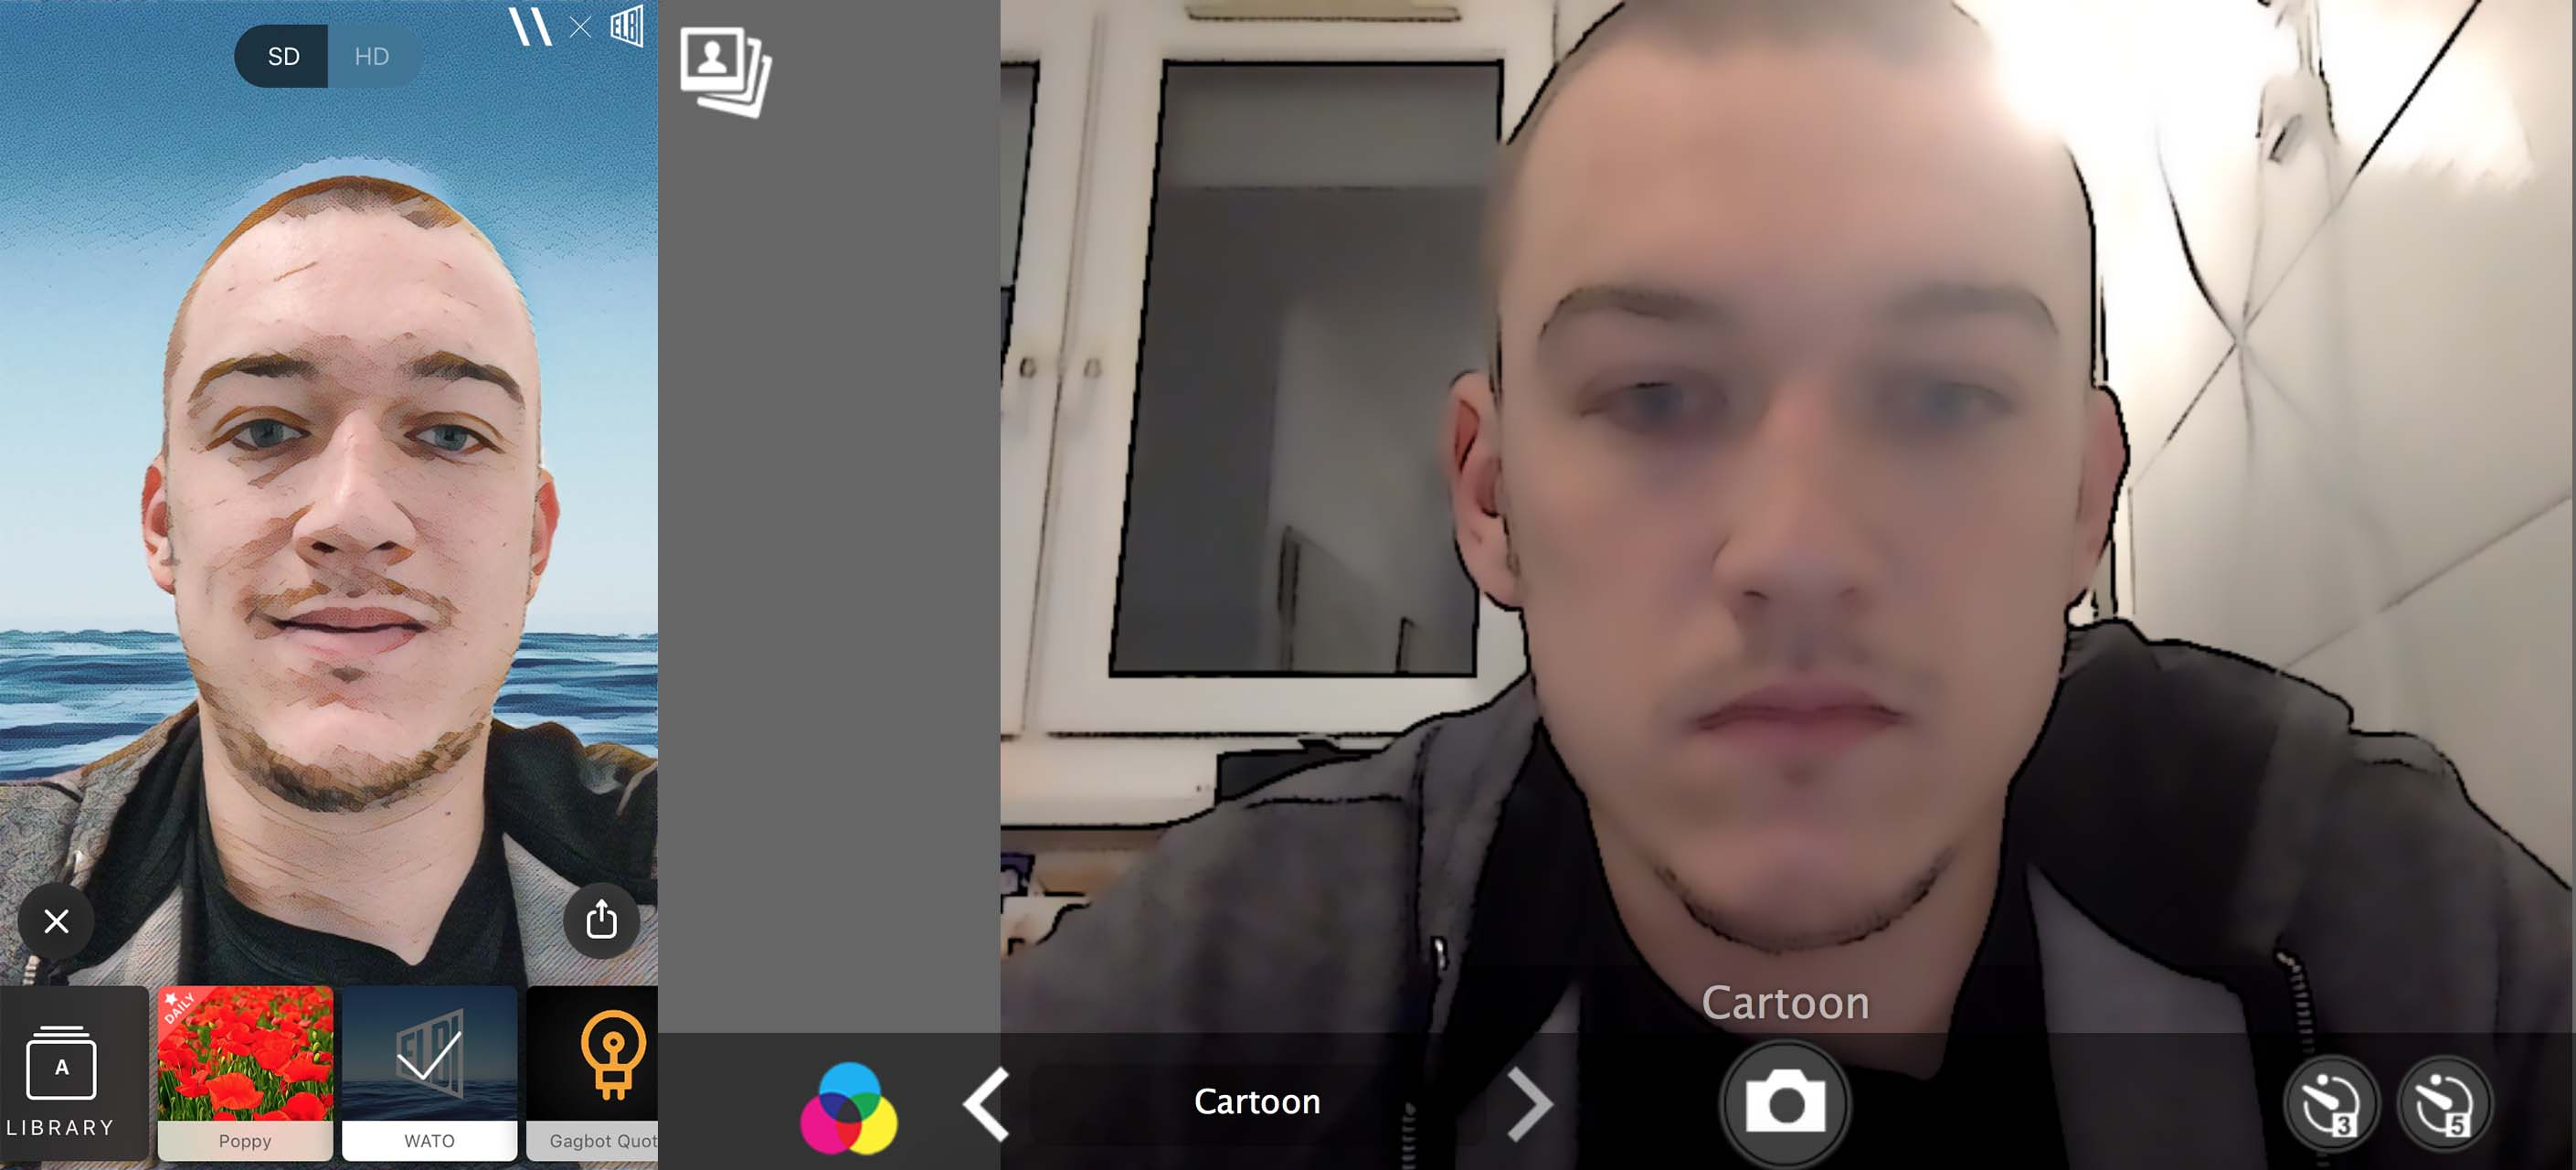
\epsfig{file=kepek/prismawebcam.jpg,scale=0.3}
\caption{Példa a Prisma és a \texttt{https://www.pixect.com} alkalmazások által készített művészi szűrőkkel ellátott képekre.} 
\label{fig:prisma}
\end{figure}

\SubSection{Filmek, játékok amelyekhez művészi szűrőket használtak}

Művészi jellegű szűrőket nem csak magánfelhasználók használnak arra, hogy érdekesebbé tegyék az elkészült fényképeiket, videóikat, hanem ilyen filtereket használnak videójátékok és filmek esetében is. Nézzünk meg ezekre is néhány példát!

\paragraph{Jet Set Radio videójáték} 

A \textit{Jet Set Radio} volt a világon az első olyan videójáték amelyen sötét árnyalatú grafikákat mutattak be, túlzott alakokkal, vastag vonalakkal és lapos, élénk színekkel \cite{jetset}. Ezzel olyan érzetet keltve, mint ha egy képregény vagy egy rajzfilm lenne. A játékban egy görkorcsolyázó karaktert lehet irányítani és graffitiznie kell a megadott helyekre mielőtt lejár az idő. Plusz pontokért lehet mindenféle extrém trükköt is csinálni korcsolyázás közben. Nehezítésként a játékost üldözik gyalogosan, helikopterekkel és tankokkal.

\paragraph{Kamera által homályosan (A Scanner Darkly) című film} 

A \textit{Kamera által homályosan} című filmet digitálisan forgatták, majd interpolált rotoszkóp segítségével animálták \cite{scannerdarkly}\cite{porthu}. Ez egy olyan animációs technika, melyben az eredeti felvételekből képkockáról képkockára filtereztek. Ezzel olyan hatást értek el, hogy azt lehet mondani erre a filmre, hogy animációs film. A film a közeljövőben játszódik. A lakosság nagy része drog fogyasztó. Beépített titkos ügynökökkel és különböző megfigyelési rendszerekkel próbálnak rendet tartani. Az egyik detektívnek, Frednek kiadják parancsba, hogy álljon rá egy nagyon veszélyes kábítószert terjesztőre, Bob Arctor-ra. A drog hatása az, hogy az emberek személyisége két, egymással ellentétes felére bomlik. Kiderül, hogy Arctor igazából Fred alteregója, igy ez az ügy elég nagy kihívásokkal jár. 
% Port.hu irodalom jegyzék 

Az említett videójátékról és filmről \aref{fig:jetset}. ábrán láthatunk egy-egy képet.

\begin{figure}[ht]
\centering
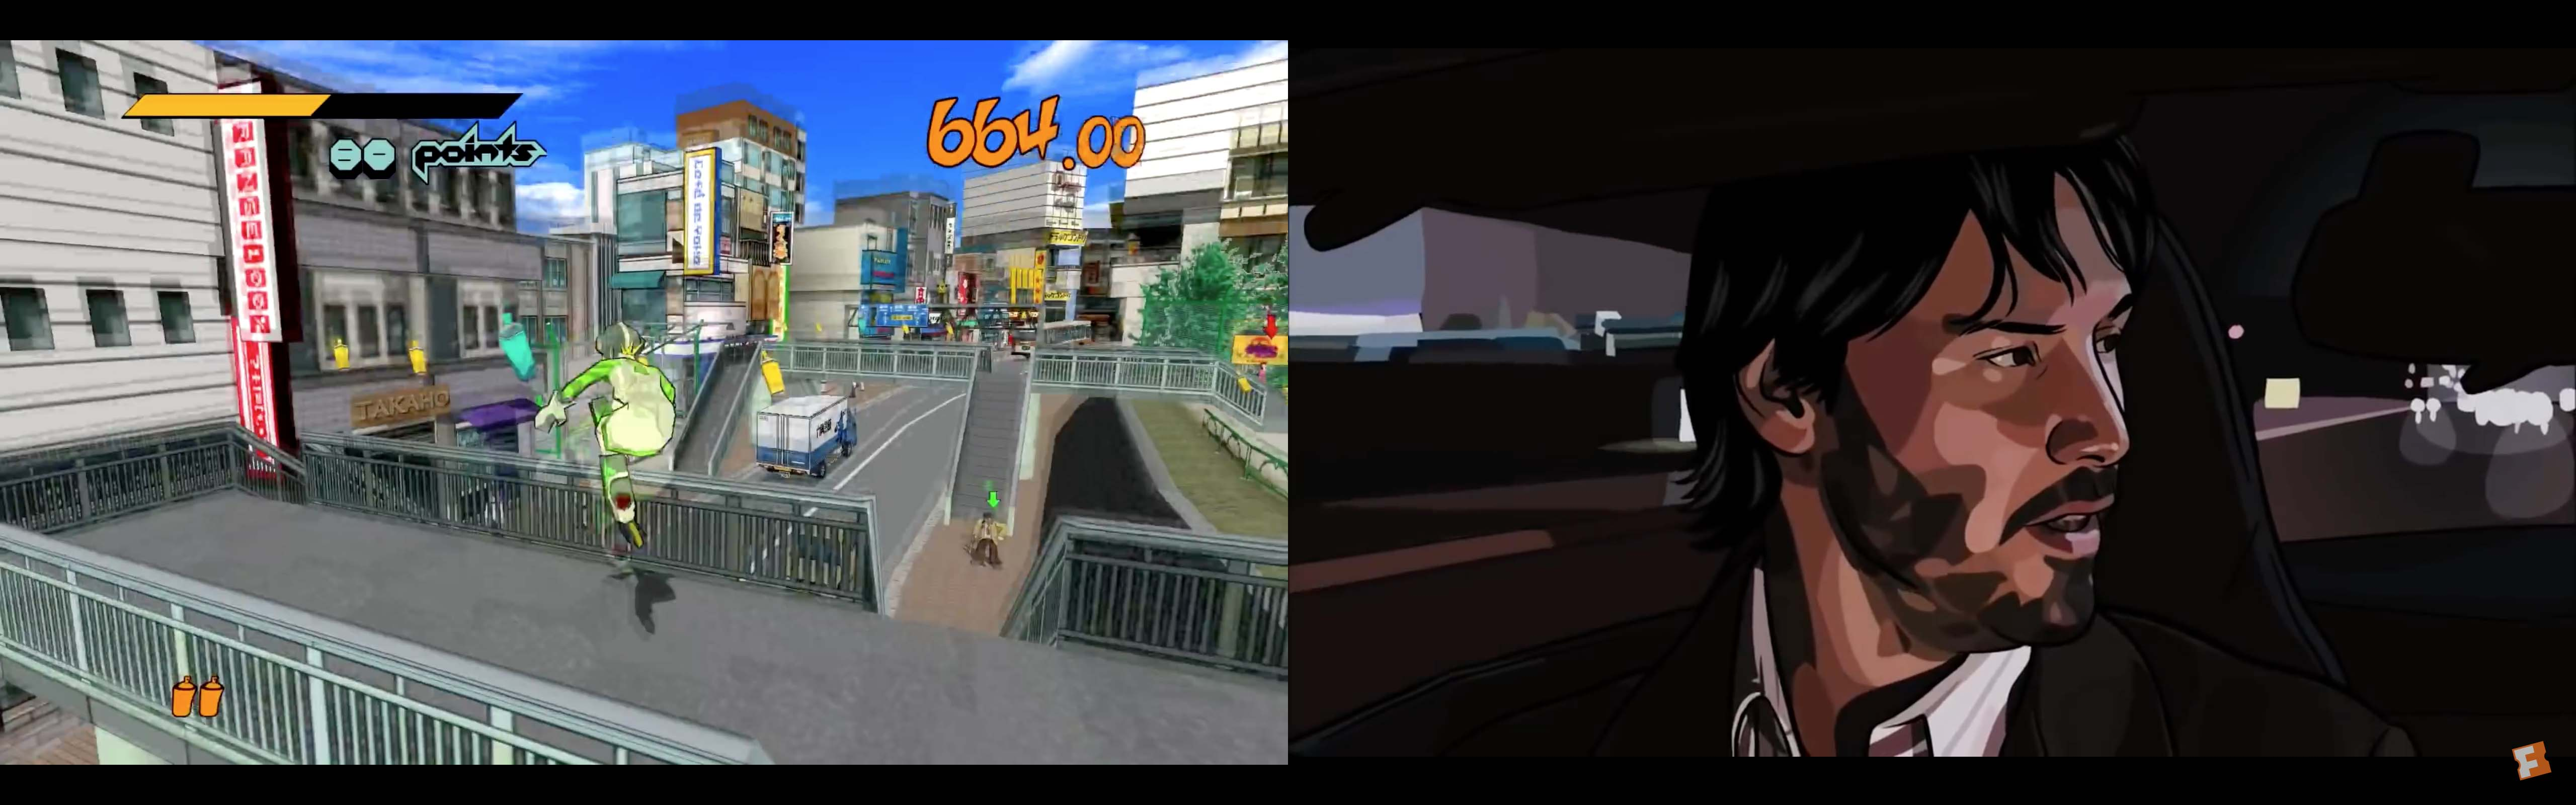
\epsfig{file=kepek/jatekfilm,scale=0.17}
\caption{Jet Set Radio videójáték és Kamera által homályosan c. film egy-egy jellegzetes képkockája} 
\label{fig:jetset}
\end{figure}

\Section{A megvalósítás nehézségei}

A digitális képfeldolgozás számítógépes algoritmusokat használ a digitális képek készítéséhez. Ez lehetővé teszi, hogy sokkal szélesebb körű algoritmusokat alkalmazzanak a bemeneti adatokra, és ezekkel az algoritmusokkal elkerülhetők az olyan problémák, mint a zaj és a jelek torzulása a feldolgozás során. Mivel a képeket két dimenzióban definiálják, a digitális képfeldolgozást multidimenzionális rendszerek formájában lehet modellezni.  Ezekkel a képfeldolgozási algoritmusokkal lehet olyan képeket készíteni, amiket például azok az alkamazások is létrehoznak amiket ebben a fejezetben bemutattam.

%https://en.wikipedia.org/wiki/Digital_image_processing

\Section{Elvárások a szűrőkkel kapcsolatban}

Olyan szűrőket szeretnék létrehozni, amelyek hasonlóképpen működnek, mint azok az applikációk, játékok, filmek amelyeket ebben a fejezetben említettem. Rajzfilm (\textit{cartoon}) jellegű, festmény szerű, valamint ceruza rajz jellegű szűrőket szándékozok létrehozni, amelyeket képekre, videókra lehet alkalmazni. A dolgozatomban ezek számítási idejét tesztelni is fogom.

% !TEX encoding = UTF-8 Unicode

\Chapter{Matematikai eszközök}

\Section{Zaj szűréshez, elmosáshoz használatos szűrők}

A következő szakaszokban annak bemutatására kerül majd sor, hogy a tervezett művészi szűrők létrehozásához milyen matematikai apparátusra van szükség. Ez alapvetően a különféle szűrési eljárások megvalósítását takarja példákkal illusztrálva.

A módszerek digitális képfeldolgozás területén közismertnek tekinthetők. A témakör feldolgozásához Kató Zoltán \textit{Digitális képfeldolgozás} című kurzusának anyagai szolgáltak alapul \cite{kato}.

\SubSection{Átlagoló szűrő}

Az átlagoló szűrő segítségével simítani lehet a képet. A képpontok közelebb kerülnek a környezetük átlagához, azaz a kép "simább" lesz, a szűrt kép intenzitásértékei a kiinulási kép intenzitástartományában maradnak. Csökkenti a zajt, de elmossa az éleket igy homályossá teszi a képet.

\example{Itt látható a átlagoló szűrésre egy példa, egy képpont 3x3 as környezete:
$$
\frac{1}{9} \times
\begin{bmatrix}
54 &26  &32 \\ 
17 &36  &24 \\ 
11 &23  &47 
\end{bmatrix}.
$$
Egyszerű simítási technika, ahol az ablakban lévő intenzitások átlaga az új intenzitás érték: 
$$
\bar{x} =
\frac{54+26+32+17+36+24+11+23+47}{9} =
\frac{270}{9} = 30.
$$}

%http://www.tankonyvtar.hu/en/tartalom/tamop412A/2011-0063_15_gepi_latas/ch05s02.html
%Kató tanár úr jegyzet
%wikipédia

\SubSection{Gauss szűrő}

A Gauss szűrő egy bemeneti kép és egy Gauss-kernel konvoluciójával jön létre. Minden egyes képpont értéket a környékének súlyozott átlagaként számolunk úgy, hogy a képpont eredeti értékének a legnagyobb a súlya, míg a távoliak kisebb súlyt kapnak. Ez olyan elmosódást eredményez, amely jobban védi a széleket, mint más egyenletes elmosódási algoritmusok. Egy Gauss függvény egyenlete egy dimenzióban az alábbi
$$
G(x) =
\frac{1}{\sqrt{2\pi\sigma^{2}}}
\cdot e^{-\frac{x^{2}}{2\sigma^{2}}}.
$$

A Gauss függvény grafikonját \aref{fig:gauss}. ábrán láthatjuk.

\begin{figure}[ht]
\centering
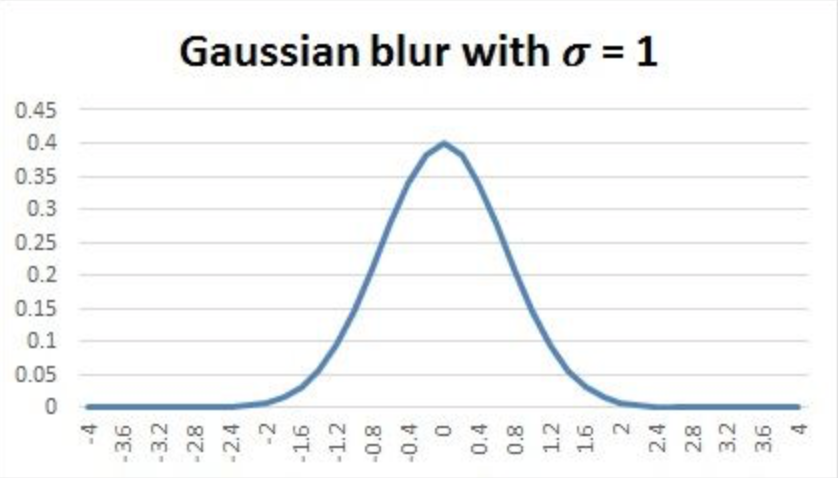
\epsfig{file=kepek/gaussgorbe.png,scale=0.65}
\caption{1 dimenziós Gauss függvény} 
\label{fig:gauss}
\end{figure}

Két dimenzióban, két Gauss együttesét kell használni, minden egyes dimenzióban: 
$$
G(x,y) =
\frac{1}{\sqrt{2\pi\sigma^{2}}} \cdot
e^{-\frac{x^{2}+y^{2}}{2\sigma^{2}}},
$$
ahol az $x$ a vízszintes tengely eredetétől való távolság, az $y$ a függőleges tengely eredetétől való távolság, a $\sigma$ pedig a Gauss eloszlás szórása. Két dimenzióban alkalmazva, ez a képlet olyan felületet hoz létre, amelynek körvonalait koncentrikus körök alkotják, a Gauss-eloszlás pedig a középpontból indul.
%wikipédia
%Kató tanár úr jegyzet
%http://fiveko.com/tutorials/image-processing/gaussian-blur-filter/

\SubSection{Medián szűrő}

Az $a_1, a_2, \dots, a_{2n+1} \in \mathbb{R}$ számok mediánja, a nagyság szerint rendezett számsorozat középső, $(n+1)$-edik eleme. Jelölhetjük például a
$med\{a_1,a_2,\dots,a_{2n+1}\}$ formában.

Teljesül rá az alábbiak:
\begin{itemize}
\item $\min\{a_i\} \leq med\{a_i\} \leq \max\{a_i\}$,
\item $\min\{a_i+c\} = med\{a_i\}+c$,
\item $med\{c\cdot a_i\}=c \cdot med\{a_i\}$.
\end{itemize}

A medián szűrést egy $S \in \mathbb{R}^2$ környezet felett a
$$
J(i,j) = med\left\{I(i+u, j+v) \mid (u, v) \in S \right\}
$$
formában végezhetjük el.

A medián szűrés eredményét az $S$ környezet mérete (és alakja) határozza meg.

\example{Itt látható a medián szűrésre egy példa, egy képpont $3 \times 3$ méretű környezete: $$
\begin{bmatrix}
54 &25  &32 \\ 
17 &37  &22 \\ 
11 &23  &45 
\end{bmatrix}.$$
Nagyság szerint sorba rendezve ezeket az értékeket, úgy hogy  11, 17, 22, 23, 25, 32, 37, 45, 54 akkor a pixel új intenzitása 25 lesz, mivel az a középső érték a sorban.}

%Kató tanár úr jegyzet
\SubSection{Kétoldalú szűrő}

A kétoldalaú szűrő egy nem lineáris, élvédő és zajcsökkentő simító szűrő a képekhez. Az egyes képpontok intenzitását a közeli pixelek intenzitásának súlyozott átlagával helyettesíti. Ez a súly Gaussian eloszláson is  alapulhat. Elengedhetetlen, hogy a súlyok nem csak az euklideszi képpontok távolságától, hanem a radiometriai különbségektől is függnek (például tartománykülönbségek, például színintenzitás, mélységi távolság stb.). Ez éles széleit megőrzi. A kétoldalú-szűrő az alábbi alakban írható föl:
\begin{align*}
I^{filtered}(x) &=
\frac{1}{W_p}\sum_{x_i\in\Omega}{I(x_i)f_r(\left \| I(x_i)-I(x) \right \|)g_s(\left \| x_i-x \right \|)}, \\
W_p &=
\sum_{x_i \in \Omega} f_r(\left \| I(x_i)-I(x) \right \|)g_s(\left \| x_i-x \right \|),
\end{align*}
ahol
\begin{itemize}
\item $I^{filtered}$ a filterrel ellátott kép,
\item $I$ az eredeti bemeneti kép,
\item $x$ a koorditánái a jelenlegi pixeleknek amik a szűrőbe kerülnek,
\item $\omega$ az ablak közepe $x$-nek,
\item $f_r$ a tartományi kernel az intenzitások közötti különbségek simítására,
\item $g_s$ a térbeli kernel a koordináták közötti különbségek simítására.
\end{itemize}
A $W_p$ súlyt a térbeli közelség és az intenzitás különbség alkalmazásával határoztuk meg. Vegyünk egy pixelt az $(i, j)$ koordinátákon, amelyet a szomszédos képpontok segítségével kell zajcsökkenteni a képen, és az egyik szomszédos pixele a $(k, l)$ helyen található. Ezután a pixelhez $(k, l)$ hozzárendelt súly az $(i, j)$ pixel zajcsökkentéséhez a következőket adja meg:
$$
w(i, j, k, l) =
\exp \left(
-\frac{(i-k)^{2}+(j-l)^{2}}{2\sigma_{d}^{2}}
-\frac{\left \| I(i,j)-I(k,l) \right \|^{2}}{2\sigma_{r}^{2}}
\right),
$$
ahol $\sigma_d$ és $\sigma_r$ a kiegyenlítési paraméterek, és $I(i, j)$ és $I(k, l)$ a pixelek $(i, j)$ és $(k, l)$ intenzitása.

A súlyok kiszámítása után normalizáljuk őket:
$$
I_{D}(i,j) =
\frac{\sum_{k,l}I(k,l)w(i, j, k, l)}{\sum_{k, l}w(i, j, k, l)},
$$
ahol az $I_D$ a pixel $(i, j)$ zajcsökkentés intenzitása.
%wikipédia

\Section{Éldetektálási módszerek}

Az éldetektálás számos matematikai módszert foglal magába, amelyek olyan pontok azonosítását célozzák meg egy képen, amelyeknél a kép fényereje élesen megváltozik. A kép egy szeletén vizsgálva az intenzitás-profilt jól azonosíthatóak az objektumok határainak megfelelő változások. Az intenzitás-gradiensből következtethetünk az élek helyére és irányára. Jellegzetes élprofilokat láthatunk \aref{fig:elprofilok}. ábrán.

\begin{figure}[ht]
\centering
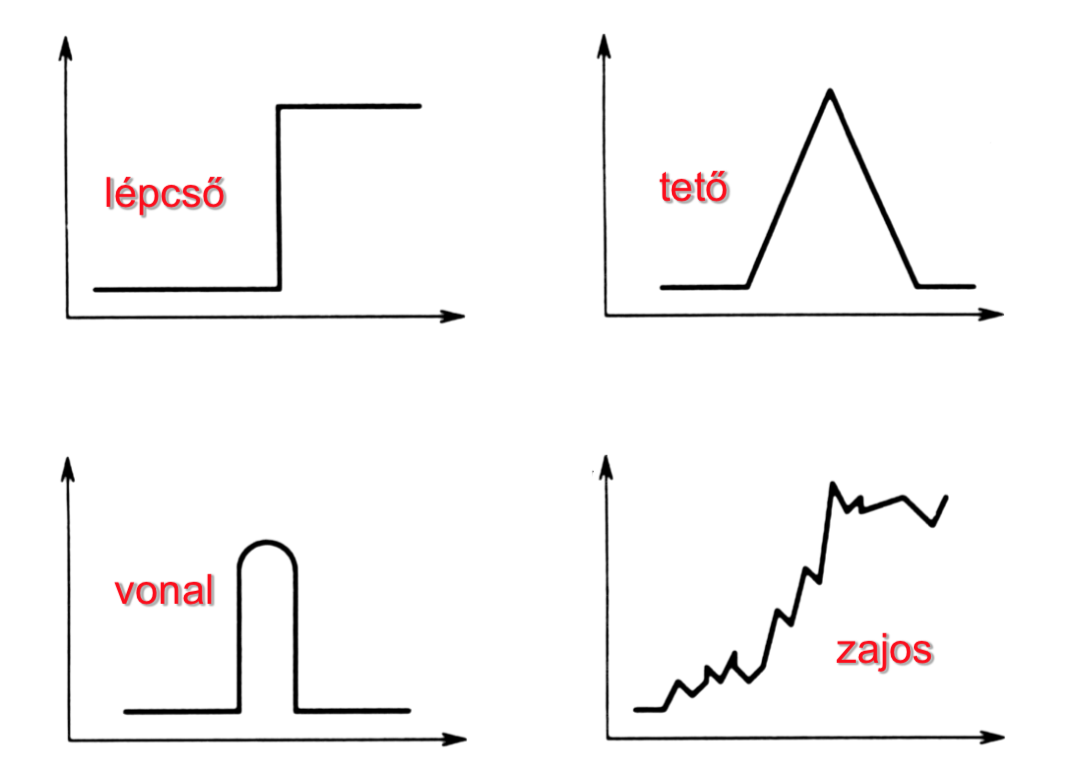
\epsfig{file=kepek/elprofilok.png,scale=0.65}
\caption{Tipikus élprofilok} 
\label{fig:elprofilok}
\end{figure}

A képfüggvény kétváltozós, tehát parciális deriváltakból álló gradiens vektoraink vannak: 
$$
\nabla f =
\left[ \genfrac{}{}{0pt}{}{G_x}{G_y} \right] =
\left[ \frac{\partial f}{\partial x}, \frac{\partial f}{\partial y}  \right]^{T.}$$
A hossza a változás nagyságával egyenlő: 
$$
\left\| \nabla f \right \| =
\sqrt{G_{x}^{2}+G_{y}^{2}} \approx
\left | G_x  \right |+\left | G_y  \right |.
$$
A gradiens a legnagyobb változás irányába mutat: 
$$
\theta = \tan^{-1}\left(\frac{G_y}{G_x}\right).
$$

Digitális képek esetén a pontos, kétváltozós függvényünk nem ismert, ezért a gradiens vektort véges differenciával közelíthetjük:
$$
\frac{\partial f}{\partial x} =
\lim_{\varepsilon \to 0} \left(
\frac{f(x+\varepsilon,y)}{\varepsilon}-\frac{f(x+y)}{\varepsilon}
\right) \approx
\frac{f(x_{n+1}+y)-f(x_n,y)}{\Delta x}.
$$

A gradiens közelítéséhez konvolúciós maszkot is használhatunk.

%Kató tanár úr jegyzet
%wikipédia

\SubSection{Sobel éldetektálás}

% TODO: Roberts éldetektálást is megemlíteni!

A Sobel éldetektáló egy gradiens alapú módszer. Ez elsőrendű deriváltakkal működik. A kép első deriváltját külön számítja az $x$ és $y$ tengelyekhez. A deriváltak csak közelítések (mivel a képek nem folytonosak). Ezek közelítéséhez az alábbi kernelt használják a konvolúcióhoz:
$$\begin{bmatrix}
-1&0  &1 \\ 
-2&0  &2 \\ 
-1&0  &1 
\end{bmatrix} 
\qquad
\begin{bmatrix}
-1&-2  &-1 \\ 
0&0  &0 \\ 
1&2  &1 
\end{bmatrix}
$$
Az első mátrix a vízszintes, a második mátrix a függőleges kernel. A bal oldali kernel megközelíti a deriváltat az $x$ tengely mentén, a jobb oldali pedig az $y$ tengely mentén. Ezen információk felhasználásával számíthatjuk ki az alábbiakat:
\begin{itemize}
\item magnitudója vagy "erőssége" az élnek: $\sqrt{G_{x}^{2}+G_{y}^{2}}$,
\item megközelítő erősség: $ \left\| G_x \right \| + \left\| G_y \right \|$,
\item az él iránya: $arctan(\frac{G_y}{G_x})$.
\end{itemize}

%Kató tanár úr jegyzet
%http://aishack.in/tutorials/sobel-laplacian-edge-detectors/

\SubSection{Laplace éldetektálás}

A Laplace éldetektáló csak egy kernelt használ. Másodfoku deriváltakat számol ki egy lépésben. Itt van néhány elterjedt kernel:
$$\begin{bmatrix}
 0 & -1  & 0 \\ 
-1 &  4  &-1 \\ 
 0 & -1  & 0 
\end{bmatrix} 
\qquad
\begin{bmatrix}
-1 & -1 & -1 \\ 
-1 &  8 & -1 \\ 
-1 & -1 & -1 
\end{bmatrix}
$$
Az első mátrix a laplace operátor, a második mátrix a laplace operátor átlókkal.

Használhatjuk akár csak az egyiket, vagy ha jobb közelítést szeretnénk, létrehozhatunk egy 5x5-ös kernelt (aminek a középpontja 24, és minden más -1).

Egy komoly hátrány azonban van, mivel másodfokú deriváltakkal dolgozunk, a laplace éldetektáló rendkívül érzékeny a zajokra. Általában zajcsökkentés szükséges. Néhány fontos további jellemzője:
\begin{itemize}
\item elmosódott élek esetén pontosabb lokalizálást érhetünk el,
\item ebben az esetben csak az élek helyét tudjuk meghatározni, az irányát nem,
\item az operátor nem érzékeny az elforgatásra.
\end{itemize}

%Kató tanár úr jegyzet
%http://aishack.in/tutorials/sobel-laplacian-edge-detectors/

\SubSection{Canny éldetektálás}

Az Canny éldetektálás olyan technika, amely a különböző objektumokból származó hasznos strukturális információkat kivonja, és drasztikusan csökkenti a feldolgozandó adatok mennyiségét. Számos számítógépes képfeldolgozó rendszerben széles körben alkalmazzák. Canny úgy találta, hogy viszonylag hasonlóak a különféle éldetektálás alkalmazására vonatkozó követelmények. Így a követelményeknek megfelelő éldetektáló megoldás számos helyzetben megvalósítható. 
\\ \\
\textbf{Algoritmus:}\\ \\
\indent 1. Gauss simítás\\
\indent 2. A kép intenzitás gradiensének megkeresése\\
\indent 3. Nem-maximumok elhagyása\\
\indent 4. Hiszterézis küszöbölés \\ 
\\
\textbf{1. Gauss simítás:}\\ \\
Mivel az éldetektálás eredményeit a képzaj is könnyen befolyásolja, elengedhetetlen a zaj kiszűrése, hogy megelőzze a zaj által okozott hamis detektálást. A kép simítása érdekében Gauss szűrőt alkalmazunk. Ez a lépés enyhén simítja a képet, hogy csökkentse a nyilvánvaló zaj hatását a éldetektálásra.
\\ \\
\textbf{2. A kép intenzitás gradiensének megkeresése:}\\ \\
A kép élei különböző irányokban jelennek meg, így a Canny algoritmus négy szűrőt használ a vízszintes, függőleges és átlós élek detektálásához az elmosódott képen. Éldetektáló operátor (például Sobel) az első derivált értékét vízszintes irányban $(G_x)$ és a függőleges irányba $(G_y)$ adja vissza. Ebből meghatározható az él-gradiens és az irány:
$$
G = sqrt{G_{x}^{2}+G_{y}^{2}},
\quad
\Theta = arctan2\left(\frac{G_y}{G_x}\right)
$$
ahol $G$ a hypot függvény segítségével számítható ki, és az arctan2 az arctangens függvény két argumentummal.

Az élirány-szög négy függőleges, vízszintes és két átlós (0 , 45 , 90  és 135 fokok) függőleges szögek egyikére kerekítve van. Az egyes színsávokba eső élek iránya meghatározott szögértékekre van beállítva.

\textbf{3. Nem-maximumok elhagyása:}

A nem-maximumok elhagyása a "vékony" élekre alkalmazzák. A gradiens kiszámítása után a gradiens értékből kivont él még mindig homályos. A 3. kritérium vonatkozásában csak egy pontos válasz lehet az élre. Így a nem-maximumok elhagyása segíthet elhagyni a gradiens értékeket (0-ra állítva), kivéve a lokális maximumokat, amelyek a legerősebb intenzitásérték-változást jelzik. Az algoritmus a következő, minden pixelre a gradiens képen:
\begin{itemize}
\item Hasonlítsa össze az aktuális képpont él-erősségét a pixel él-erősségével, pozitív és negatív gradiens irányba.
\item Ha az aktuális képpont él-erőssége a legnagyobb az azonos irányú maszk más képpontjaihoz képest, az érték megmarad. Ellenkező esetben az érték elhagyásra kerül.
\end{itemize}

Bizonyos implementációkban az algoritmus a folyamatos gradiens irányokat különálló diszkrét irányokba sorolja, majd egy $3 \times 3$ szűrőt rak az előző lépés kimenetre. Minden pixelben elhagyja a középső képpont él-erősségét (az értékét 0-ra állítva), ha nagysága nem nagyobb, mint a két szomszéd nagysága a gradiens irányba.

\textbf{4. Hiszterézis küszöbölés:}

Eddig az erős élű képpontokat minden bizonnyal be kell vonni a végső élbe, mivel ezek a kép valódi éleiből származnak.Vannak azonban viták a gyenge élű képpontokról, mivel ezek a pixelek kiválaszthatók az igazi élről, vagy a zaj/színváltozatokról. Pontos eredmény elérése érdekében az utóbbi okok által okozott gyenge éleket el kell távolítani. Általában gyenge él pixeleket okoznak, az igazi élek amikor erős élű pixelekhez kapcsolódnak, amíg a zajok nem kapcsolódnak hozzá. Az élkapcsolat nyomon követéséhez a blob elemzést kell végre hajtani, ami egy gyenge élű pixel és 8-as kapcsolatú szomszédos pixelek figyelembevétele. Mindaddig, amíg van egy erős élű pixel, amely részt vesz a blob elemzésben, a gyenge élű pontot lehet azonosítani, amit meg is kell őrizni.

%Kató tanár úr jegyzet
%wikipédia

\Section{Szegmentálás}

Számítógépes látásmódban a képszegmentálás a digitális kép több szegmensbe való felosztása. A szegmentálás célja egyszerűsíteni és/vagy megváltoztatni a kép reprezentációját ezzel könnyebbé téve a kép elemzését. A kép szegmentálását általában objektumok és határok megtalálásához használják. Pontosabban, a képszegmentálás egy címke hozzárendelését jelenti a kép minden képpontjához úgy, hogy az azonos címkével rendelkező pixelek bizonyos tulajdonságokkal rendelkeznek. A képszegmentáció eredménye olyan szegmensek csoportja, amelyek együttesen fedik le a teljes képet vagy a képből kinyert kontúrt. Valamennyi régióban lévő pixelek hasonlóak bizonyos jellemzők vagy számított tulajdonságok, például szín, intenzitás vagy textúra tekintetében. A szomszédos régiók szignifikánsan különböznek az azonos jellegzetességek tekintetében.

%wikipédia

\SubSection{Mean shift algoritmus}

Mean shift egy eljárás a maximális értékek azonosítására, ahol a sűrűségfüggvény módjait a funkciótól vett diszkrét adat szolgáltatja. Ez egy iteratív módszer, az $x$ kezdeti becslésével kezdünk. Adjuk meg a $K(x_i - x)$ kernel függvényt. Ez a függvény határozza meg a közeli pontok súlyát az átlag újraértékeléséhez. Általában egy Gaussian kernelt használunk az aktuális becsléshez képest, $K (x_i - x) = e ^ {- c || x_i - x || ^ 2}$. A $K$ által meghatározott ablak sűrűségének súlyozott átlaga: 
$$
m(x) =
\frac{\sum_{x_i \in N(x)}K(x_i-x)x_i}{\sum_{x_i \in N(x)}K(x_i-x)},
$$
ahol $N(x)$ az $x$ szomszédsága, olyan pontok halmaza, amelyekhez $K(x_ {i}) \neq 0$.

Az $m (x) -x$ különbséget az Fukunaga és a Hostetler átlagos eltolódásának nevezik. Az mean shift algoritmus most beállítja az $x \leftarrow m(x)$ értéket, és megismétli a becslést, amíg $m(x)$-ig konvergál.

\Section{Küszöbölés}

% TODO: Érdemes lehet még az éldetektálás elé rakni!

A küszöbérték a képszegmentálás legegyszerűbb módja. A szürkeárnyalatos képből küszöbérték használatával bináris képek készíthető. Tételezzük fel, hogy az objektum és a háttér eltérő intenzitású, vagyis nagy a kontraszt. Az objektum és a háttér önmagában homogén intenzitású. A küszöbölést így a hisztogram alapján választott megfelelő értékkel el tudjuk végezni (\ref{fig:threshold}. ábra).

Zajos kép esetén nehéz kielégítő köszöbértéket meghatározni, tehát a szegmentálás inhomogén lesz, erre a zajszűrés jelenthet megoldást.

%wikipédia

\begin{figure}[ht]
\centering
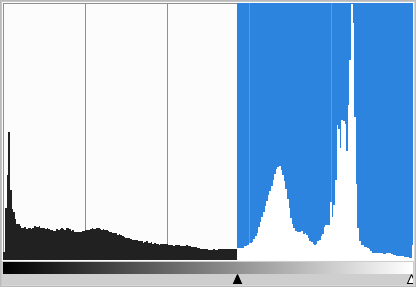
\epsfig{file=kepek/threshold.png,scale=0.65}
\caption{Példa a hisztogram alapján egy megfelelő küszöbérték megválasztására} 
\label{fig:threshold}
\end{figure}

% TODO: Az alábbit még át kell majd kicsit fogalmazni!

\example{Sötét objektum világos háttérben:\\
$f(x,y)$- bemeneti kép;\\
$t(x,y)$- szegmentált kép;\\
$T$=küszöbérték\\
\\
$f(x,y)\leq T$, akkor $t(x,y)=1$, azaz objektum.\\
$f(x,y)> T$, akkor $t(x,y)=0$, azaz háttér.
}\\\\
Léteznek adaptív eljárások, melyek az input képhez automatikusan választják ki az optimális küszöbértéket. Ebből vannak globális és lokális küszöbértéket meghatározó algoritmusok. A globális köszöbölésre alkalmas algoritmusok hisztogramból klaszterezéssel számított értékekel dolgoznak. Ilyen például az Isodata valamint az Otsu algoritmus. A lokális küszöbölés változó értékekkel dolgozik, például egyenletlen megvilágítás. Amennyiben az objektum és a háttér kontrasztja globális küszöbölés után, lokálisan még mindig nagy, akkor alkalmazzuk a lokális küszöbölést, például Niblack algoritmust.

%Kató tanár úr jegyzet
%wikipédia

\SubSection{Izodata algoritmus (Yanni)}

Jól használható, ha az előtér és a háttér körülbelül ugyanannyi képpontból áll. Az algoritmus az alábbi lépésekből áll.
\begin{itemize}
\item[1.] Inicializálás: a hisztogramot kétrészre osztjuk, célszerűen a felezőponton: $T_0$
\item[2.] Kiszámítjuk az objektum valamint a háttér intenzitásának a középértékét: $M_i, m_i$
\item[3.] Az új küszöbérték a két középérték átlaga: $T_i=(M_i+m_i)/2$
\item[4.] Vége ha a küszöbérték már nem változik: $T_k+1=T_k$
\end{itemize}

%Kató tanár úr jegyzet

\SubSection{Otsu algoritmus}

A bemeneti kép $L$ szürkeárnyalatot tartalmaz, a normalizált hisztogram minden $x$ szürkeértékéhez megadja az előfordulási gyakoriságát, vagyis a valószínűségét: $p_x$. Keressük azt a $T$ küszöbszámot, amely maximalizálja az objektum-háttér közötti varianciát.

\textbf{Az előtér/háttér pixelek gyakorisága és középértéke:}

Háttér valószínűsége:
$$
B(T) = \sum\limits_{x=1}\limits^{T}p_x 
$$

Objektum valószínűsége:
$$
1-B(T)=\sum\limits_{x=T+1}\limits^{L}p_x
$$

Legyen $m(T)\equiv \sum\limits_{x=1}\limits^{T}xp_x$, a teljes kép középértéke: $\mu \equiv m(L) = \sum\limits_{x=1}\limits^{L}xp_x$,

Háttér középértéke:
$$
\mu_B =\frac{m(T)}{B(T)}
$$

Objektum középértéke:
$$
\mu_O =\frac{\mu-m(T)}{1-B(T)}\\
$$

\textbf{Az előtér/háttér pixelek szórása:}

$$
\sigma^2_B =
\frac{1}{B(T)}\sum\limits_{x=1}\limits^{T}(x-\mu_B)^2 p_x,
$$
$$
\sigma^2_O =
\frac{1}{1-B(T)}\sum\limits_{x=T+1}\limits^{L}(x-\mu_O)^2 p_x
$$

\textbf{A teljes kép szórása:}
$$
\sigma^2 =
\sum_{x=1}^T(x-\mu)^2 p_x + \sum_{x=T+1}^L(x-\mu)^2 p_x =
\dots =
$$
$$
= B(T)\sigma_B^2+(1-B(T))\sigma_O^2 + (\mu_B-\mu)^2B(T)+(\mu_O-\mu)^2(1-B(T)) \equiv \sigma^2_W(T)+\sigma^2_C(T)
$$
ahol, a $B(T)\sigma_B^2+(1-B(T))\sigma_O^2 = \sigma^2_W(T)$, osztályon belüli varianciától függ és a $(\mu_B-\mu)^2B(T)+(\mu_O-\mu)^2(1-B(T)) = \sigma^2_C(T)$, osztályokközötti varianciától függ. A $\sigma^2$ konstans, és $T$-t úgy kell beállítani, hogy $\sigma_C^2(T)$ a lehető legnagyobb legyen:
$$
\sigma^2_C(T) = \dots = \frac{(\mu(T)-\mu B(T))^2}{B(T)(1-B(T))}
$$
A hisztogram elejéről kezdve nézzük meg minden szürkeértéket, mint lehetséges küszöböt. Kiszámoljuk a $\sigma^2_C(T)$ értéket a $\mu(T)$ és $B(T)$  segítségével, mindaddig növeljök a $T$ értékét, amíg $\sigma^2_C(T)$ kövekszik. Ez az algoritmus feltételezi, hogy $\sigma^2_C(T)$-nek egy maximuma van.

%Kató tanár úr jegyzet

\SubSection{Niblack algoritmus}

Egyetlen küszöb nem elegendő az objektum és a háttér szétválasztásához. Ezért változó köszöbérték $(T(i,j))$ kell, amely követi az intenzitás változásokat:
$$
T(i,j)=\mu(i, j) + k \sigma(i, j)
$$
Az $(i,j)$ adott környezetében, $\mu(i,j)$ a középértéket jelenti, $\sigma(i, j)$ pedig a szórást. A $k$ egy súly, ami megmutatja mennyire vegyük figyelembe a szórást.

Ha $k < 0$, akkor sötét az objektum,
Ha $k > 0$, akkor világos az objektum.

A változó küszöbértékre láthatunk egy szemléltetést \aref{fig:niblack}. ábrán.

\begin{figure}[ht]
\centering
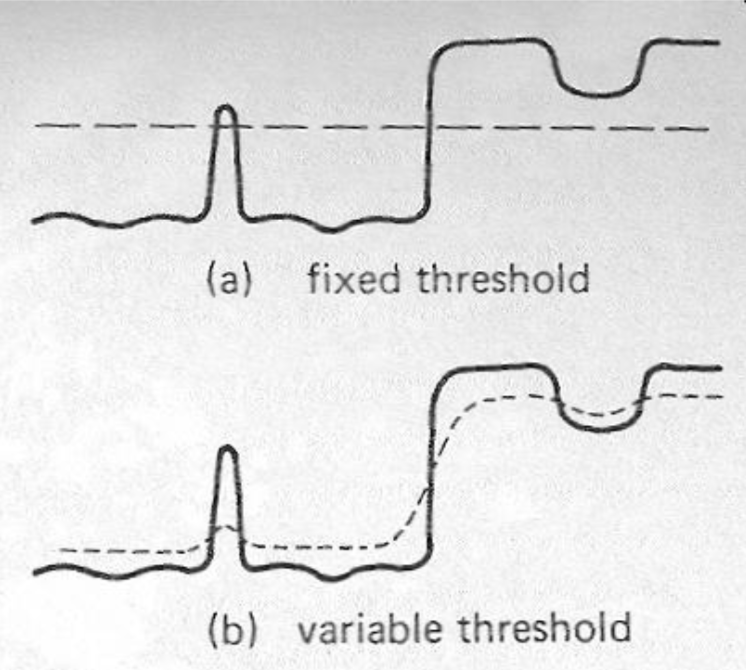
\epsfig{file=kepek/niblack.png,scale=0.65}
\caption{Változó küszöbérték} 
\label{fig:niblack}
\end{figure}

%Kató tanár úr jegyzet

% !TEX encoding = UTF-8 Unicode

\Chapter{Szűrő algoritmusok}
Ebben a fejezetben azokat a filtereket szeretném részletezni, amelyeket megírtam C++ progaramozási nyelven. Ezek többségükben cartoon, valamint festmény jellegűek. A szűrőket nem csak képeken teszteltem, hanem videókon is és valós időben is a számítógépem kamerájával, de azok eredményét majd a \textbf{6. fejezet}ben fogom bővebben kifejteni.
\Section{Cartoon-style filter}
Az első filter egy Cartoon-style filter, amely az éleket kiemeli és a színeket elmossa. Ezekhez a műveletekhez Gauss-piramist, kétoldalú szűrést, medián szűrést illetve adaptív küszöbölést használtam.
\begin{figure}[ht]
\centering
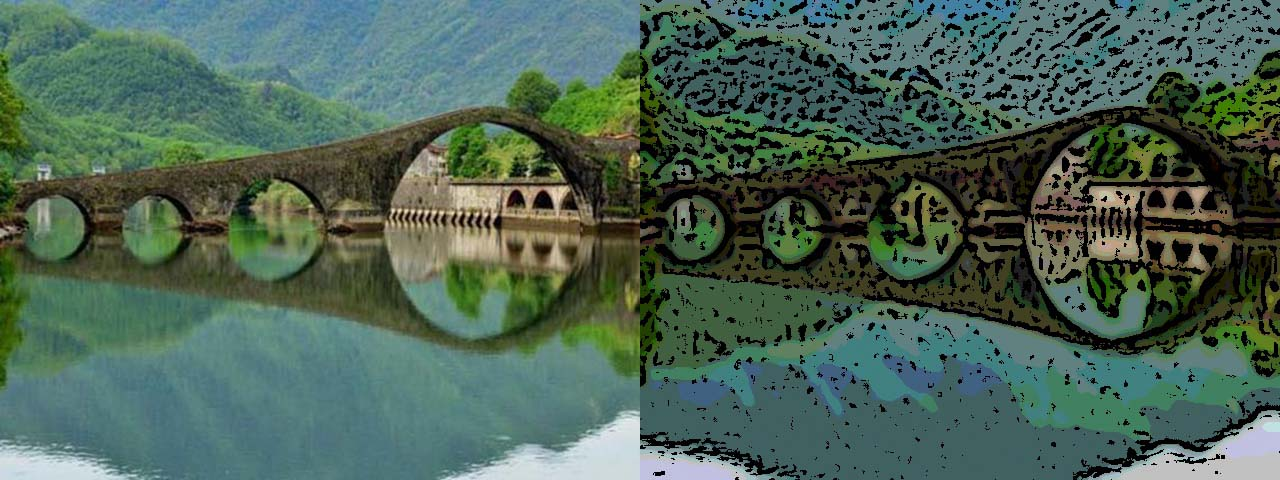
\epsfig{file=kepek/1_cartoon_filter.jpg, width=15cm, height=5.625cm}
\caption{Bal oldalon az eredeti kép látható, jobb oldalon a filterrel ellátott kép} 
\label{fig: cartoon1}
\end{figure}
\SubSection{Gauss-piramis és kétoldalú szűrő}
Első lépésben az eredeti képet lekicsinyítettem Gauss-piramis segítségével a kép méretének negyedére, rátettem egy kétoldalú szűrőt, majd vissza nagyítottam az eredeti méretre. A Gauss-piramis a kép kicsinyítése előtt Gauss-simítás segítségével súlyoz. A kétoldalú szűrő egy nem lineáris, élvédő és zajcsökkentő simító szűrő.
\begin{figure}[ht]
\centering

\epsfig{file=kepek/pyrambilateral.jpg,scale=0.45}
\caption{A Gauss-piramisban kicsinyítés és nagyítás valamint a kétoldalú szűrő eredménye } 
\label{fig: cartoon2}
\end{figure}

\SubSection{Színek konvertálása, medián szűrő}
Ebben a lépésben először az előzőleg kapott elmosott, színes képet átkonvertáltam szürkeárnyalatos képpé. 
Itt kiszeretnék térni egy kicst magára a színes kép szürkeárnyalatossá konvertálására, mert eddig a dolgozatomban nem került szóba. Több féle megoldás létezik, ebből párat megemlítenék, az egyik az RGB komponensek átlagolása, de ez az emberi szem számára pontatlan, mivel nem egyformán érzzékel minden színt. A következő megoldás amit az OpenCV- beépített színkonvertálása is használ az, hogy minden színkomponenst súlyoz. A harmadik megoldás pedig, HSV színrendszerben alakítja át a képet szűrkeárnyalatossá. Ebben az esetben az OpenCV-s beépített kovertálást használtam a súlyok pedig a következők: 
$$\text{RGB to Gray} = 0.299\cdot R+0.587\cdot G+0.114\cdot B.$$ 
Ennek eredményeként kapott képen medián szűrést hajtottam végre, amit ismét zajcsökkentés miatt alkalmaztam. Így a kép már teljesen el van mosva, egyre jobban cartoon hatása van.
\begin{figure}[ht]
\centering
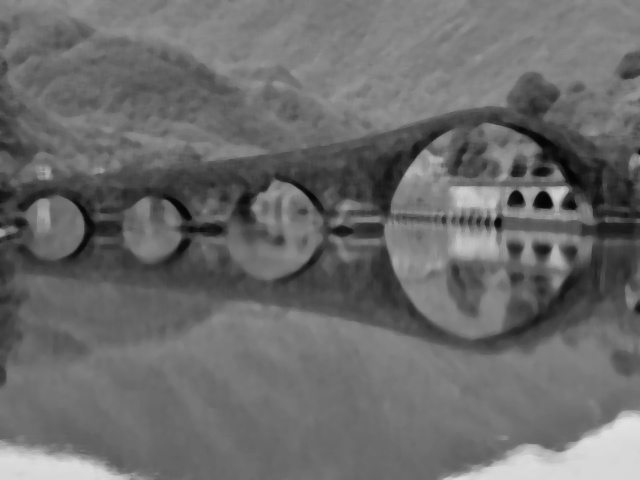
\epsfig{file=kepek/graymedian.jpg,scale=0.45}
\caption{Szürkére átalakított kép medián szűrővel } 
\label{fig: cartoon3}
\end{figure}
\newpage
\SubSection{Adaptív küszöbölés az élek kiemelésére}
Az adaptív küszöbérték általában szürkeárnyalatos vagy színes képet ad bemenetként, és a legegyszerűbb megvalósításban bináris képet jelenít meg. A kép minden egyes képpontjára egy küszöbértéket kell kiszámítani. Ha a képpontérték a küszöbérték alatt van, akkor a háttérértékre van állítva, ellenkező esetben az előtérbe kerül.
\begin{figure}[ht]
\centering
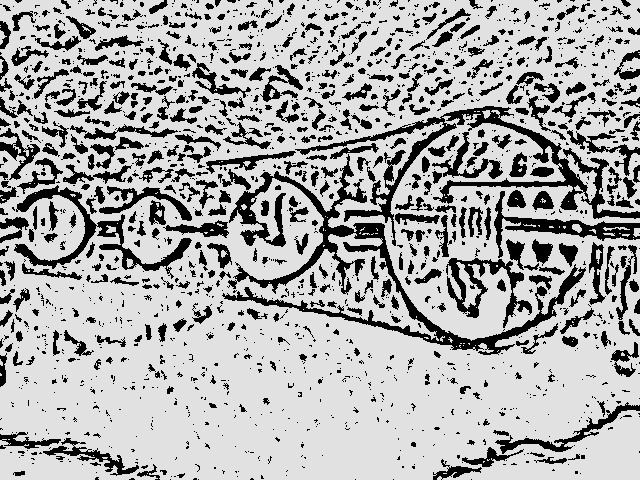
\epsfig{file=kepek/threshold.jpg,scale=0.40}
\caption{Adaptív küszöbölés  } 
\label{fig: cartoon4}
\end{figure}
\SubSection{A szűrőkkel és a köszöböléssel előállított képek eggyesítése}
Az adaptív küszöböléssel elkészült maszkot át kell konvertálni színes képpé, hogy egyesíteni tudjuk az "elmosott" képpel amit az első két lépésben hoztunk létre.
\begin{figure}[ht]
\centering
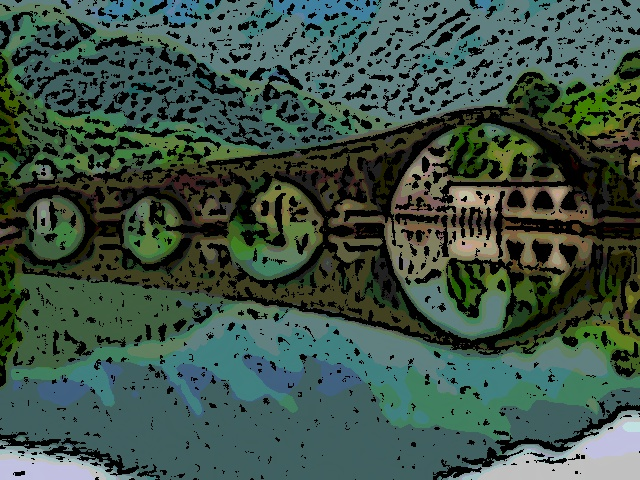
\epsfig{file=kepek/Cartoon_filter.jpg,scale=0.40}
\caption{Cartoon-style szűrő } 
\label{fig: cartoon5}
\end{figure}
%http://www.askaswiss.com/2016/01/how-to-create-cartoon-effect-opencv-python.html
\Section{Pencil sketch filter}
Megpróbáltam egy olyan algoritmust létrehozni, ami egy ceruza rajzot imitál. Ehhez szűrkeárnyalatosra konvertáltam a képet, Medián szűrőt, Gauss szűrőt és egyéb képfeldolgozási műveleteket használtam, valamint egy "vásznat" is ráraktam, hogy még jobban olyan érzete legyen a képnek mint ha rajzolták volna.
\begin{figure}[ht]
\centering
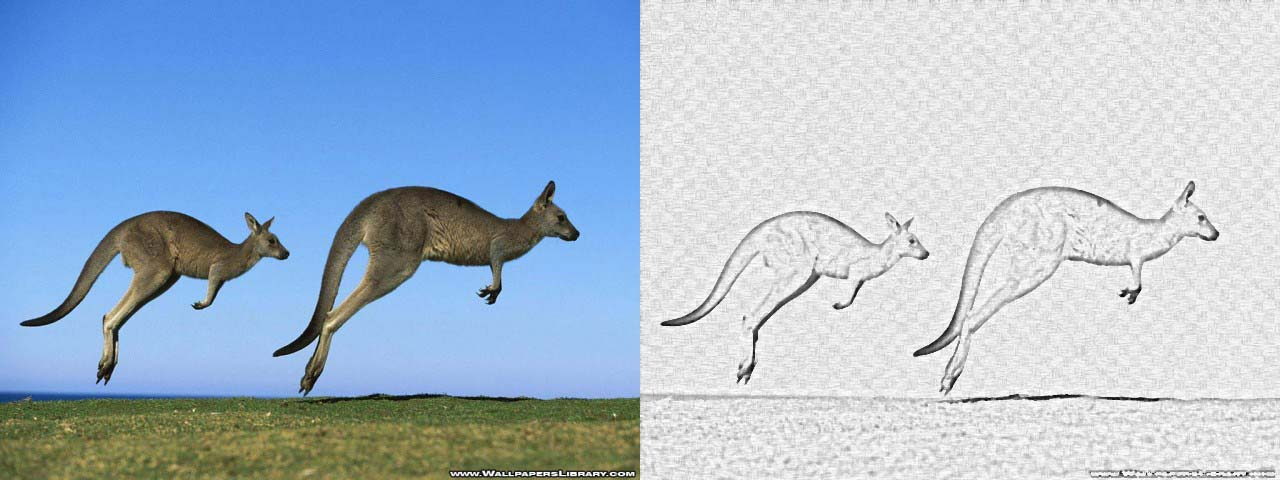
\epsfig{file=kepek/2_pencil_sketch_filter.jpg,width=15cm, height=5.625cm}
\caption{Bal oldalon az eredeti kép látható, jobb oldalon a filterrel ellátott kép } 
\label{fig: pencil1}
\end{figure}
\SubSection{Medián szűrő}
A kép szűrkeárnyalatos konvertálása után, végrehajtottam egy medián szűrést annak érdekében, hogy kiszűrjük az apróbb zajokat.
\begin{figure}[ht]
\centering
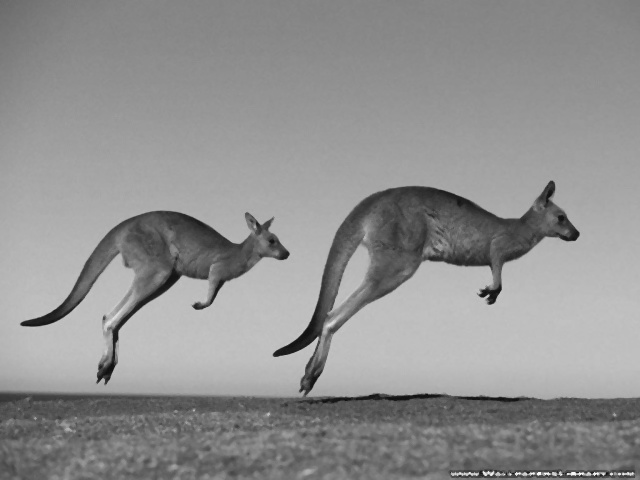
\epsfig{file=kepek/mediangray.jpg,scale=0.50}
\caption{Szürkére átalakított kép medián szűrővel  } 
\label{fig: pencil2}
\end{figure}
\SubSection{Gauss szűrő}
Ezt a simítási teknikát, a képzaj  és a részletesség csökkentése érdekében használtam. Olyan sima elmosódást eredményez a képen, mint ha a nem lenne fókuszban.
\begin{figure}[ht]
\centering
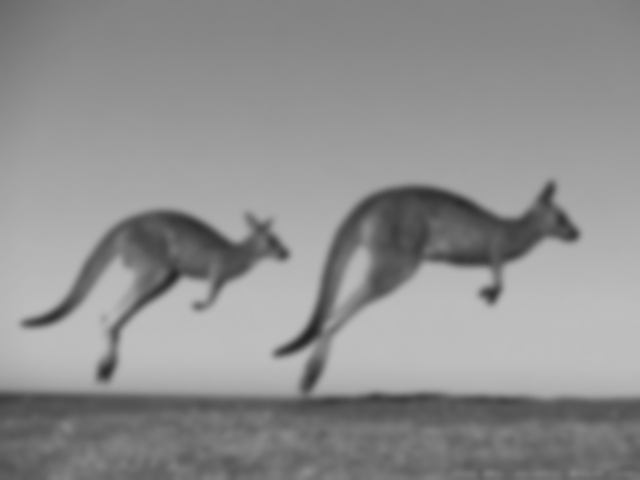
\epsfig{file=kepek/gauss.jpg,scale=0.43}
\caption{Gauss szűrő használata } 
\label{fig: pencil3}
\end{figure}
\SubSection{Az előző két lépés elosztása }
Az előző két szűrőt elosztottam egymással, így már tényleg majdnem olyan képet kaptam ami már ceruza rajz szerű. Úgy gondoltam még azért ráfér némi javítás, így még további műveleteket hajtottam végre rajta.
\begin{figure}[ht] 
\centering
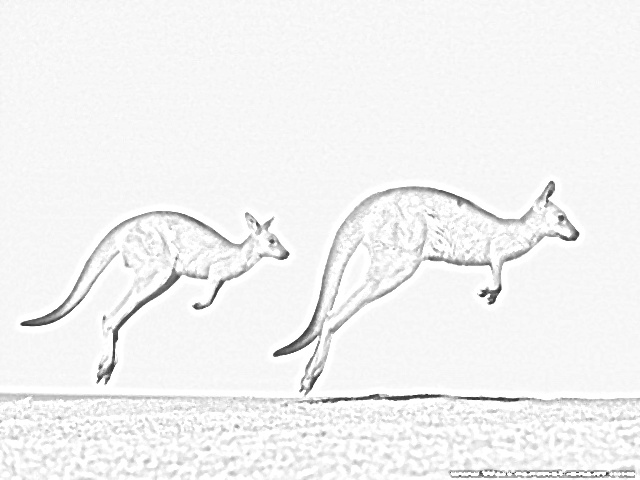
\epsfig{file=kepek/blend.jpg,scale=0.43}
\caption{Medián szűrés és a Gauss szűrés hányadosa } 
\label{fig: pencil4}
\end{figure}
\SubSection{Kontraszt széthúzása}
Azt figyeltem meg, hogy ha így hagyom a "Pencil sketch" szűrőt, akkor némely képen eléggé kontraszt szegény. Így úgy gondoltam rakok bele egy kontraszt széthúzást, hogy még kontrasztosabb legyen a kép. A  kontraszt széthúzásról még nem beszéltem, a kontraszt széthúzás vagy másnéven normalizáció egy egyszerű képjavító eljárás, amely megpróbálja javítani a kép kontrasztját azáltal, hogy "kiterjeszti" a benne lévő intenzitásértékek tartományát a kívánt értéktartományra. 
\begin{figure}[ht]
\centering
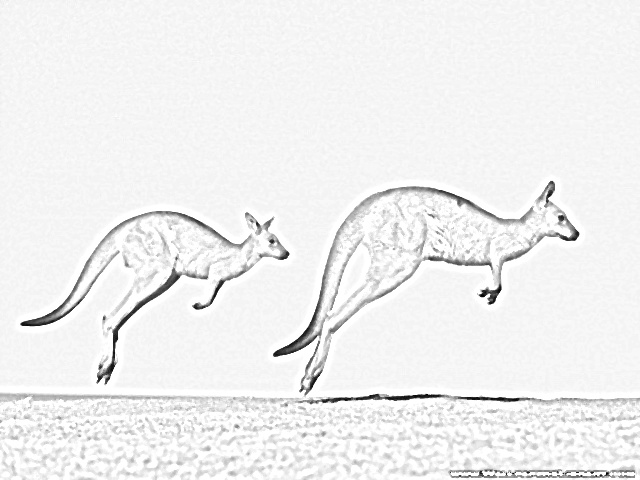
\epsfig{file=kepek/contraststrech.jpg,scale=0.50}
\caption{Kontraszt széthúzás } 
\label{fig: pencil5}
\end{figure}
\SubSection{Vászon hozzáadása}
A kontraszt széthúzása után, már egészen olyan hatása volt a képnek mint ha egy ceruza rajz lenne. Ráraktam még egy "vászont" ami személyes véleményem szerint mégjobban segíti azt az érzetet hogy ez egy ceruza rajz. Először a vászonnak a színét átkellett konvertálnom színesből szűrkeárnyalatossá, hogy használható legyen a kontraszt széthúzott képhez. Ezek után a vászont összeszoroztam eddig eredményül kapott képpel így jött létre a "Pencil sketch filter".
\begin{figure}[ht] 
\centering

\epsfig{file=kepek/canvasgray.jpg,width=10cm, height=3cm}
\caption{Vászon színének konvertálása } 
\label{fig: pencil6}
\end{figure}
Így készült el végeredményként ez a kép.
\begin{figure}[ht]
\centering
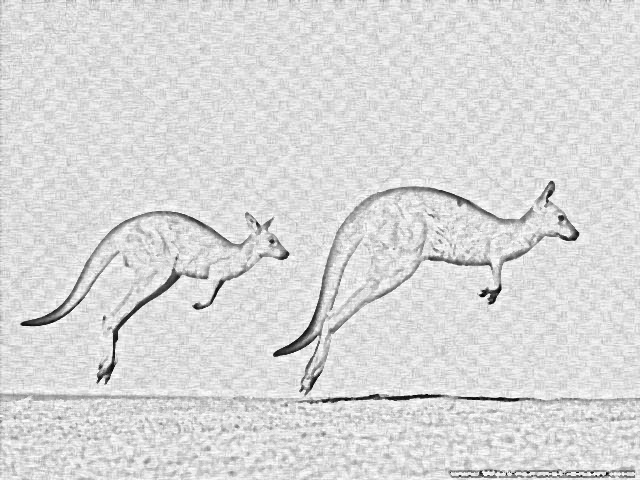
\epsfig{file=kepek/pencil_sketch.jpg, scale=0.50}
\caption{Pencil sketch filter } 
\label{fig: pencil7}
\end{figure}
\newpage
\Section{Cartoon filter}
Megpróbáltam más technikával is létrehozni egy cartoon hatású képet. Ahol medián szűrőt, Laplace éldetektálást valamit küszöbölést használtam.
\begin{figure}[ht]
\centering
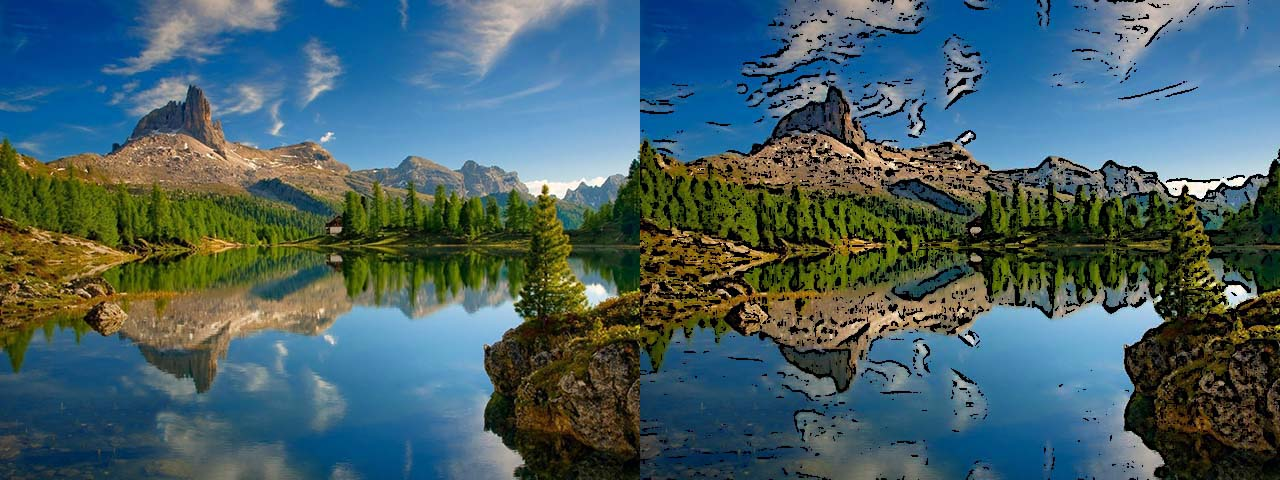
\epsfig{file=kepek/3_cartoon_filter2.jpg,width=15cm, height=5.625cm}
\caption{Bal oldalon az eredeti kép látható, jobb oldalon a filterrel ellátott kép } 
\label{fig: 2_cartoon1}
\end{figure}
\SubSection{Medián szűrő}
Mint az eddigi saját filtereknél itt is előfeldolgozásként elvégeztem szürkeárnyalatossá konvertálást valamint egy  medián szűrést. 
\begin{figure}[ht]
\centering
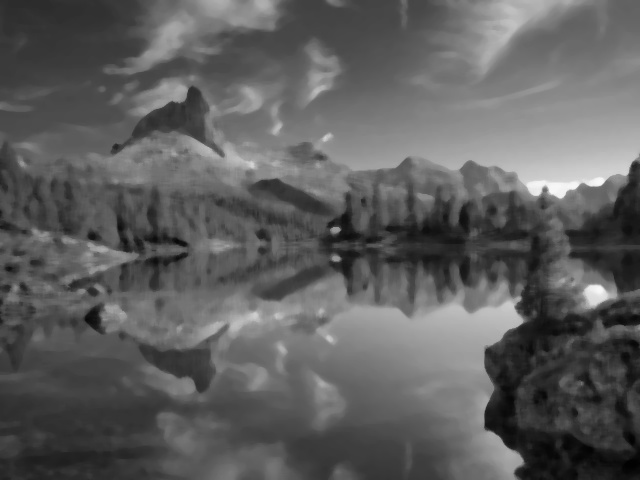
\epsfig{file=kepek/Cartoon1_gray.jpg,scale=0.485}
\caption{Szürkére átalakított kép medián szűrővel  } 
\label{fig:  2_cartoon2}
\end{figure}
\SubSection{Laplace éldetektálás}
Ennél a filternél a Laplace éldetektálást választottam, azért ezt a módszert mert ezzel olyan élmaszkot tudtam készíteni ami kicsit hasonló a ceruza rajzhoz. Vékony kontúrként emeli ki a képben található éleket. Ez az éldetektálás gradiensekkel számol, ahol a gradiens nagy, ott a második derivált 0.
\begin{figure}[ht]
\centering
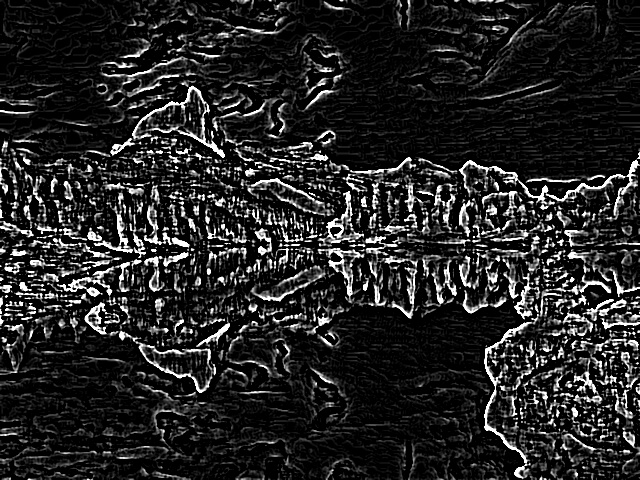
\epsfig{file=kepek/Cartoon1_laplacian.jpg,scale=0.485}
\caption{Laplacian éldetektálás  } 
\label{fig:  2_cartoon3}
\end{figure}
\SubSection{Küszöbölés}
Az éldetektálás után, alkalmaztam egy küszöbölést amivel létrejött egy maszk, amit összeraktam az eredeti képpel.
\begin{figure}[ht]
\centering

\epsfig{file=kepek/Cartoon1_thresh.jpg,scale=0.4}
\caption{Küszöbölés  } 
\label{fig:  2_cartoon4}
\end{figure}
Így készült el végeredményként a Cartoon filter.
\begin{figure}[ht]
\centering
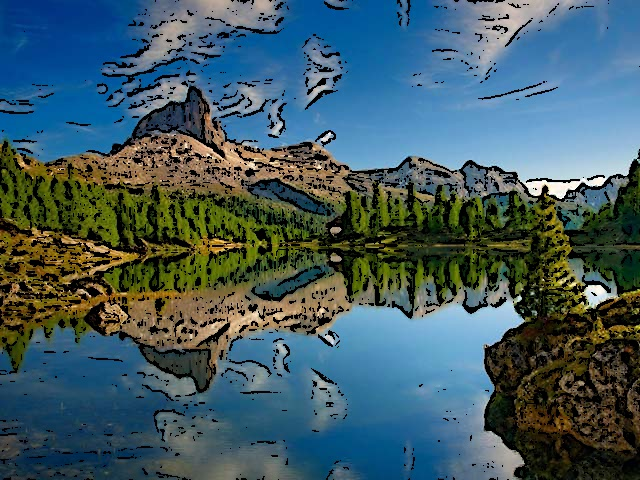
\epsfig{file=kepek/Cartoon1_filter1.jpg,scale=0.48}
\caption{Cartoon filter  } 
\label{fig:  2_cartoon4}
\end{figure}
%https://github.com/MasteringOpenCV/code/blob/master/Chapter1_AndroidCartoonifier/Cartoonifier_Desktop/cartoon.cpp
\newpage
\Section{Aquarelle-style filter}
Az utolsó saját szűrő amit készítettem az egy egyszerű aquarell hatású szűrő. Ez a szűrő teljesen más technikával készült mint az eddigiek. Nem használtam éldetektálást illettve küszöbölést sem. Az eredeti képpel dolgoztam végig nem maszkoltam. Azért is egyszerű mert igazából két lépéssel megoldható, elég egy átlagoló szűrés és egy mean shift szegmentálás.
\begin{figure}[ht]
\centering

\epsfig{file=kepek/4_paint_filter.jpg,width=15cm, height=5.625cm}
\caption{Aquarelle-style filter} 
\label{fig:  paint}
\end{figure}
\SubSection{Átlagoló szűrő}
Átlagoló szűrővel elmostam az eredeti színes képet, hogy az apróbb zajokat kiszűrjem.
\begin{figure}[ht]
\centering

\epsfig{file=kepek/Paint_filter_blur.jpg,scale=0.48}
\caption{Átlagoló szűrő  } 
\label{fig: paint1}
\end{figure}
\SubSection{Mean shift szegmentálás }
Minden egyes adatpontnál a mean shift meghatároz egy ablakot, és kiszámítja az adatpont átlagát. Ezután az ablak közepét az átlag felé tolja, és megismétli az algoritmust, amíg konvergens. Az mean shift egy nemparametrikus iteratív algoritmus vagy egy nemparametrikus sűrűségi gradiens becslés egy általánosított kernel megközelítés alkalmazásával.
\begin{figure}[ht]
\centering

\epsfig{file=kepek/Paint_filter.jpg,scale=0.48}
\caption{Aquarelle-style filter, mean shift szegmentálás  eredménye} 
\label{fig: paint1}
\end{figure}
%https://gist.github.com/dgym/5532135
% Ide kellene felsorolni majd a saját szűrők algoritmusait!
% !TEX encoding = UTF-8 Unicode

\Chapter{Implementáció C++ és OpenCV segítségével}
\Section{OpenCV bemutatása}

Az OpenCV (Open Source Computer Vision Library) egy nyílt forráskódú számítógépes látás és gépi tanulási szoftverkönyvtár. Az OpenCV-t azért hozták létre, hogy közös infrastruktúrát biztosítson a számítógépes megjelenítési alkalmazások számára, és felgyorsítsa a gépi érzékelés használatát a kereskedelmi termékekben. BSD licenc alatt került kiadásra, ezért ingyenes mind tudományos, mind kereskedelmi célokra. C ++, Python és Java interfészekkel rendelkezik, és támogatja a Windows, Linux, Mac OS, iOS és Android rendszereket. Az OpenCV-et a számítási hatékonyságra tervezték, és nagy hangsúlyt fektetett a valós idejű alkalmazásokra. Az optimalizált C / C ++-ban írt, a könyvtár kihasználhatja a többmagos feldolgozást is. Az OpenCL használatával kihasználhatja az alapul szolgáló heterogén számítási platform hardveres gyorsítását.
\\

\noindent A könyvtár több mint 2500 optimalizált algoritmussal rendelkezik, amely magába foglalja mind a klasszikus, mind a legmodernebb számítógépes látásmódot és a gépi tanulási algoritmusokat. Ezek az algoritmusok felismerhetik az arcokat, felismerhetik az objektumokat, osztályozhatják az emberi cselekvéseket a videókban, nyomon követhetik a mozgásokat, követhetik a mozgó objektumokat, eltávolíthatja a vörös szemeket a vakuval készített képekből, követheti a szemmozgásokat, felismerheti a tájat stb. 
\\
%https://opencv.org
\Section{Beépített művészi jellegű OpenCV-s szűrők}
Az OpenCV könyvtár rendelkezik saját bepített, nem fotorealisztikus szűrőkkel, amelyeknél csak a bemeneti képet, valamint néhány paramétert kell megadnunk a függvénynek és ő elkészíti nekünk a filterezett képet. Négy ilyen beépített függvény található az OpenCV-ben, Edge Preserving filter, Detail Enhancing filter, Pencil sketch filter és a Stylization filter. Ezek C++ implementációját szeretném bemutatni.
\SubSection{Edge Preserving filter}
Az első ilyen szűrő az Edge Preversing filter, ami az éleket megörzi de a hátteret elmossa. 
\begin{cpp}
edgePreservingFilter(Mat src, Mat dst, int flags=1, 
			float sigma_s=60, float sigma_r=0.4f);
\end{cpp}
ahol, \textbf{src} a bemeneti kép, amit szertnénk átalakítani,\\
\indent \textbf{dst} a filterrel ellátot kép, \\
\indent \textbf{flags} maga az él kiemelő filter melynek két paramétere lehet, \textbf{RECURS\_FILTER} (rekurív szűrő) aminek az értéke 1 vagy \textbf{NORMCONV\_FILTER} (normalizált konvolúció) aminek az értéke 2.  A futási sebességtől függ melyik paramétert alkalmazzuk, ha gyorsabb sebességet akarounk elérni akkor a rekurzív filtert alkamazzuk, ha viszont nem számít a sebesség akkor a  normalizált konvolúciót mert az szebben kiemeli az éleket.\\
\indent \textbf{sigma\_s} egy skála 0 és 200 között, Sigma\_spatial a simítás mértékét határozzuk meg, \\
\indent \textbf{sigma\_r} egy skála 0 és 1 között, Sigma\_range szabályozza, hogy a szomszédságon belül a különböző színek milyen mértékben átlagolódjanak.
\begin{figure}[ht]
\centering
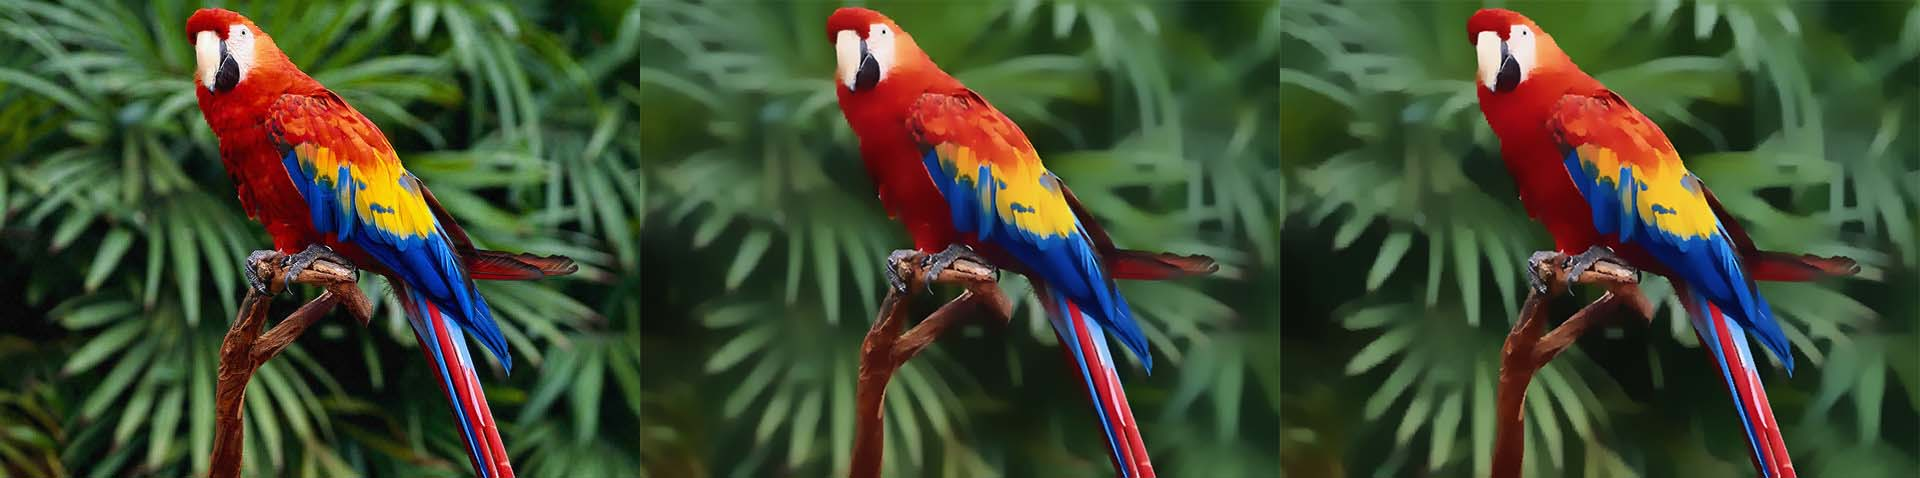
\epsfig{file=kepek/edgePreservingFilter.jpg,scale=0.45}
\caption{Eredeti kép, Rekurzív filter, Normalizált konvolúció} 
\label{fig: edgePreservingFilter}
\end{figure}
\SubSection{Detail Enhancing filter}
A második ilyen szűrő a Detail Enhancing filter, ami a képet élesebbé teszi.
\begin{cpp}
detailEnhance(Mat src, Mat dst, float sigma_s=10, float sigma_r=0.15f);
\end{cpp}
A paraméterek megegyeznek az Edge Preserving filter paramétereivel. 
 \begin{figure}[ht]
\centering
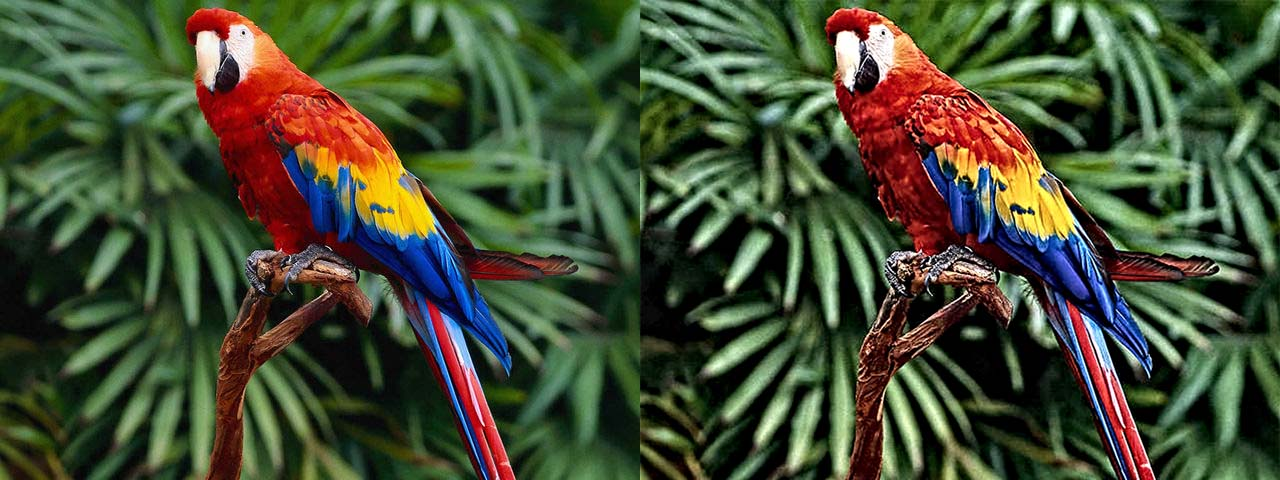
\epsfig{file=kepek/detailEnhance.jpg,scale=0.65}
\caption{Eredeti kép, Detail Enhancing filter eredménye} 
\label{fig:detailEnhance}
\end{figure}
\SubSection{Pencil sketch filter}
Ez a szűrő ceruza rajzot eredményez, két féle képet eredményez egy színes képet és egy szürkeárnyalatosat.
\begin{cpp}
pencilSketch(Mat src, Mat dst_gray, Mat dst_color, float sigma_s=60, 
		float sigma_r=0.07f, float shade_factor=0.02f);
\end{cpp}
A paraméterek megegyeznek az Edge Preserving szűrőével, de bővül egy paraméterrel.\\
\indent \textbf{shade\_factor}  ami egy 0 és 0,1 közötti érték, a kimeneti képintenzitás skálázása. Minél magasabb az érték, annál fényesebb az eredmény.
\begin{figure}[ht]
\centering
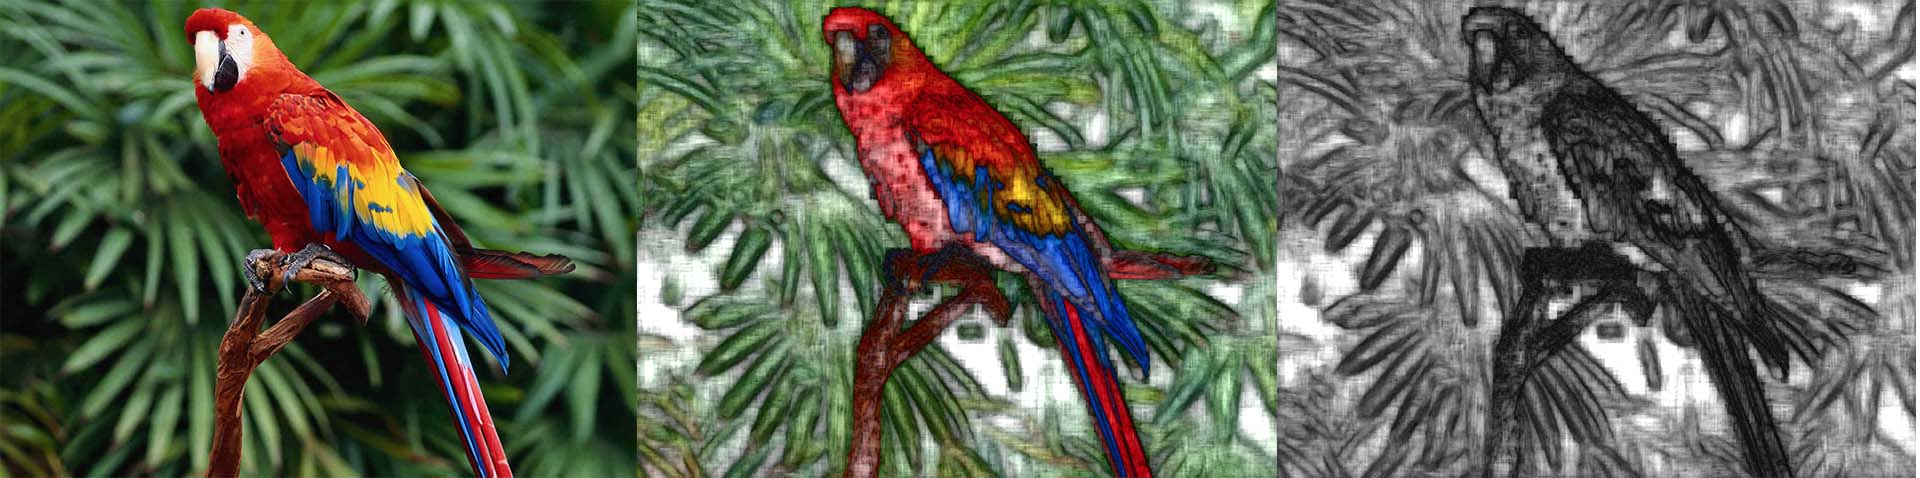
\epsfig{file=kepek/pencil_sketch_color_grey.jpg,scale=0.45}
\caption{Eredeti kép, Pencil sketch filter színes, Pencil sketch filter szűrkeárnyalatos} 
\label{fig: pencil_sketch_color_grey}
\end{figure}
\SubSection{Stylization filter}
A Stylization filter olyan kimeneti képet eredményez, aminek olyan hatása van mint ha vízfestékkel készítették volna.
\begin{cpp}
stylization(Mat src, Mat dst, float sigma_s=60, float sigma_r=0.45f);
\end{cpp}
A paraméterek megegyeznek az Edge Preserving filter paramétereivel. 
 \begin{figure}[ht]
\centering
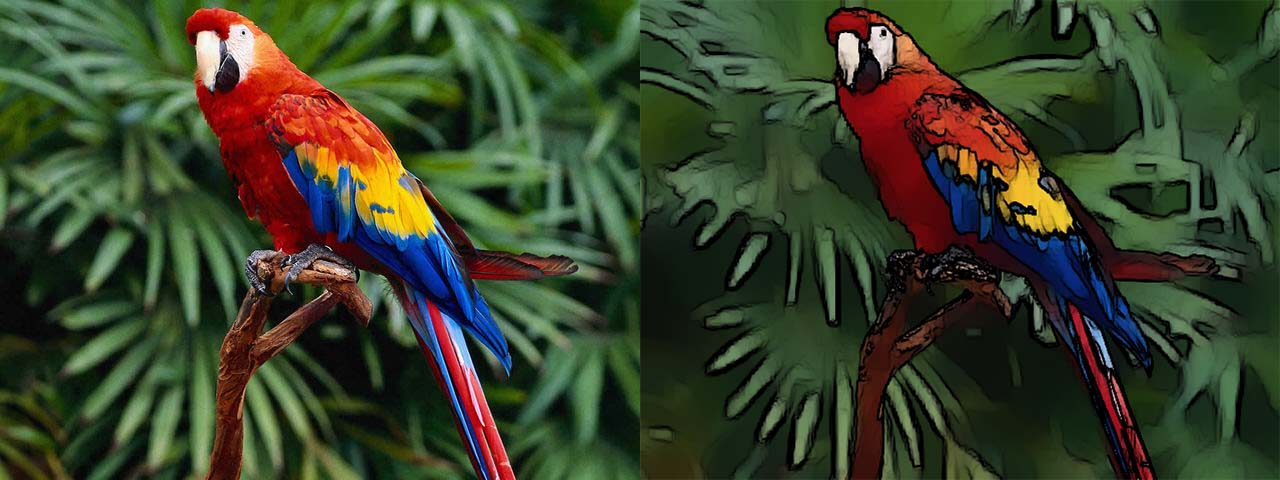
\epsfig{file=kepek/stylization.jpg,scale=0.65}
\caption{Eredeti kép, Stylization filter eredménye} 
\label{fig: stylization}
\end{figure}
%https://www.learnopencv.com/non-photorealistic-rendering-using-opencv-python-c/
\Section{Saját szűrők implementációja OpenCV és C++-al}
Ebben a fejezetben szeretném bemutatni a saját szűrőknek a C++ implementációját és a paramétereket amiket használtam hozzájuk. Itt képekkel nem fogok illusztrálni, mert azok a \textbf{4. fejezetben} megtalálhatóak. \\ Elsőként bemutatnám a kép betöltésének implementációját, amit minden szűrőn használtam.
\begin{cpp}
    Mat img = imread("image.jpg"); // bemeneti kep
    Mat dst ; //kimeneti kep
    //Ha valami nem stimmel a kep betoltesnel
    if ( img.empty() )
    {
        cout << "Error loading the image" << endl;
        return -1;
    }
\end{cpp} 
Ablak létrehozása :
\begin{cpp}
    namedWindow("Original image", 1);
    namedWindow("Image with filter", 1);
\end{cpp}
Ezután következik az a rész, amit a következő alfejezetekben fogok részletezni, hogy tulajdon képpen milyen lépésekből épül fel a filter. \\
Ezek után a kép megjelenítése:
\begin{cpp}
    imshow("Original imagel",img );
    imshow("Image with filter", dst);
\end{cpp} 
\newpage
\noindentÉs végezetül a waitKey funkció következik, amely a megadott milliszekundumban megjeleníti a képet. Mivel itt nem mozgó képről beszélünk igy az értéke 0.
 \begin{cpp}
    waitKey(0);
\end{cpp}
\SubSection{Cartoon-style filter}
Gauss piramisban lefelé lépünk kettőt.
\begin{cpp}
 for(int i=0; i < 2;i++){
    pyrDown( img, img);
    }
\end{cpp}
ahol, \\
\indent \textbf{img}: a bemeneti színes kép,\\
\indent \textbf{img}: a kimeneti kicsinyített színes kép.\\\\
Egymás után 7 szer hajtjuk végre a kétoldalú szűrőt.
\begin{cpp}
Mat img_res;
int d = 9;
double sigmaColor = 9.0;
double sigmaSpace = 7.0;
for(int i=0; i < 7;i++){
    bilateralFilter ( img, img_res, d, sigmaColor, sigmaSpace );
    }
\end{cpp}
ahol, \\
\indent \textbf{img}: a bemeneti színes kép,\\
\indent \textbf{img\_res}: a kimeneti kép kétoldalú szűrővel,\\
\indent \textbf{d}: a szűrés során használt minden egyes pixel szomszédság átmérője. Ha nem pozitív, akkor kiszámítható a sigmaSpace-ből,\\
\indent \textbf{sigmaColor}: szűri a szigmát a színtérben ,\\
\indent \textbf{sigmaSpace}: szűri a szigmát a koordinátatérben.\\ \\
Gauss piramisban felfelé lépünk kettőt, hogy visszanyerjük az eredeti kép méretet.
\begin{cpp}
 for(int i=0; i < 2;i++){
    pyrUp( img_res, img_res);
    }
\end{cpp}
ahol, \\
\indent \textbf{img\_res}: a bemeneti kép kétoldalú szűrővel,\\
\indent \textbf{img\_res}: a kimeneti nagyított színes kép.\\\\
Kép konvertálása szürkeárnyalatossá. 
\begin{cpp}
cvtColor(img, srcGray, CV_BGR2GRAY);
\end{cpp}
ahol, \\
\indent \textbf{img}: a bemeneti színes kép,\\
\indent \textbf{srcGray}: a kimeneti szürkeárnyalatos kép,\\
\indent \textbf{CV\_BGR2GRAY}: színes kép szürkeárnyalatosra alakítására használatos paraméter.\\ \\
A következő lépésben a medián szűrőt implementáltam.
\begin{cpp}
int kernel_size = 7;
medianBlur(srcGray, median, kernel_size );
\end{cpp}
ahol, \\
\indent \textbf{srcGray}: a bemeneti szürkeárnyalatos kép,\\
\indent \textbf{median}: a kimeneti medián szűrővel ellátott kép,\\
\indent \textbf{kernel\_size}: a kernel mérete, itt ebben az esetben egy $7 x 7$-es mátrix. Ami már nem csak a zaj kiszűrését eredményezi, hanem már cartoon jellegűre mossa a képet.\\ \\
Adaptív küszöbölés implementációja.
\begin{cpp}
Mat img_edge;
double maxValue = 225;
int blockSize = 9;
double C = 2; 
adaptiveThreshold(median,img_edge, maxValue, ADAPTIVE_THRESH_MEAN_C,
		THRESH_BINARY,blockSize,C); 
\end{cpp}
ahol, \\
\indent \textbf{median}: a bemeneti medián szűrővel ellátott kép,\\
\indent \textbf{img\_edge}: a kimeneti éldetektálás eredménye,\\
\indent \textbf{maxValue}: nem zérus érték hozzárendelve azokhoz a képpontokhoz, amelyekhez a feltétel teljesül.\\ 
\indent \textbf{ADAPTIVE\_THRESH\_MEAN\_C}: adaptiv küszöbölés algoritmus,\\
\indent \textbf{THRESH\_BINARY}: a küszöbérték típusának THRESH\_BINARY vagy THRESH\_BINARY\_INV értékűnek kell lennie,\\
\indent \textbf{blockSize}: a pixel szomszédságának mérete, amelyet a pixel küszöbértékének kiszámítására használnak,\\
\indent \textbf{C}: a konstanst az átlagból vagy a súlyozott átlagból kell levonni, normális esetben pozitív, de lehet nulla vagy negatív is.\\\\
A maszk színesre konvertálása.
\begin{cpp}
cvtColor(img_edge, img_edge, CV_GRAY2RGB);
\end{cpp}
ahol, \\
\indent \textbf{img\_edge}: a bemeneti szürkeárnyalatos kép,\\
\indent \textbf{img\_edge}: a kimeneti színes kép,\\
\indent \textbf{CV\_GRAY2RGB}: szürkeárnyalatos kép színesre alakítására használatos paraméter.\\ \\
Az elmosott kép és a maszk egyesítése. 
\begin{cpp}
Mat img_cartoon;
bitwise_and(img_res,img_edge,img_cartoon);
\end{cpp}
ahol, \\
\indent \textbf{img\_res}: a bemeneti elmosott kép,\\
\indent \textbf{img\_edge}: a bemeneti élmaszk,\\
\indent \textbf{img\_cartoon}: kimeneti Cartoon-style filterezett kép.
\SubSection{Pencil sketch filter}
Első lépésként átkonvertáltam a képet színesről szűrkeárnyalatossá majd egy medián szűrést hajtottam végre. Ezt az előző szűrőnél már bemutattam így itt nem részletezném, annyiban változik a paraméterezése, hogy a kernel mérete itt egy $3 x 3$-as mátrix.\\
A következő lépésben egy Gauss simítást implementáltam. 
\begin{cpp}
Mat gauss;
Size ksize = Size(21, 21);
double sigmaX = 0;
double sigmaY = 0;
GaussianBlur(median, gauss, ksize, sigmaX, sigmaY);
\end{cpp}
ahol, \\
\indent \textbf{median}: a bemeneti medián szűrővel ellátott kép,\\
\indent \textbf{img\_blur}: a kimeneti Gauss szűrés eredménye,\\
\indent \textbf{ksize}: a kernel mérete, itt ebben az esetben egy $21 x 21$-es mátrix,\\
\indent \textbf{sigmaX}: a Gauss kernel standard elterese X iranyba,\\
\indent \textbf{sigmaY}: a Gauss kernel standard elterese Y iranyba.\\ \\
A medián és Gauss szűrő elosztása egymással.
\begin{cpp}
Mat img_blend;
double scale_d = 245;
divide(median, gauss, img_blend, scale_d);   
\end{cpp}
ahol, \\
\indent \textbf{median}: a bemeneti medián szűrővel ellátott kép,\\
\indent \textbf{img\_blur}: a bemeneti Gauss szűrővel ellátott kép,\\
\indent \textbf{img\_blend}: a kimeneti kép a szűrők elosztásának eredménye,\\
\indent \textbf{scale\_d}: a skalár tényező.\\ \\
Kontraszt széthúzás.
\begin{cpp}
double alpha=0; 
double beta=255;
normalize(img_blend, img_blend, alpha, beta, CV_MINMAX);
\end{cpp}
ahol,
\begin{itemize}
\item \texttt{img\_blend}: a két szűrő elosztásával kapott kép,
\item \texttt{img\_blend}: a kimeneti kontraszt széthúzással kapott kép,
\item \texttt{alpha}: normál érték a normálértékhez viszonyítva vagy az alsó tartomány határértéke esetén,
\item \texttt{beta}: első tartományhatár a tartomány normalizálása esetén,
\item \texttt{CV\_MINMAX}: választható maszk művelet.
\end{itemize}

A szürkeárnyalatos vászon összeszorzása a kontraszt széthúzott képpel.
\begin{cpp}
double scale_m = 1.0 / 256;
multiply(img_blend, canvas, img_blend, scale_m);
\end{cpp}
ahol, \\
\indent \textbf{img\_blend}: a bemeneti kontraszt széthúzással ellátott kép,\\
\indent \textbf{canvas}: a bemenet vászon képe,\\
\indent \textbf{img\_blend}: a kimeneti összeszorzott kép,\\
\indent \textbf{scale\_m}: választható skálafaktor.\\\\
\SubSection{Cartoon filter}
Első lépésként itt mint az előző filtereknél, átkonvertáltam a képet színesről szűrkeárnyalatossá majd egy medián szűrést hajtottam végre, ahol a kernel mérete $7 x 7$-es matrix.\\
Ezt egy Laplace éldetektálás követte.
\begin{cpp}
int kernel_size = 5;  
Laplacian(median, edges, CV_8U, kernel_size);
\end{cpp}
 ahol, \\
\indent \textbf{median}: a bemeneti median szűrővel ellátott kép,\\
\indent \textbf{edges}: az élekdetektálás eredménye,\\
\indent \textbf{CV\_8U}: unsigned 8bit / pixel - azaz egy pixel 0-255 értékű tartományban lehet,\\
\indent \textbf{kernel\_size}: a kernel mérete, itt ebben az esetben egy $5 x 5$-ös mátrix. Azt mutatja meg mekkora legyen a maszkon az él mérete.\\ \\
Végezetül a küszöbölés következett.
\begin{cpp}
double thresh = 90;
double maxval = 255;
threshold(edges, mask, thresh, maxval, THRESH_BINARY_INV);
\end{cpp}
 ahol, \\
\indent \textbf{edges}: a bemeneti kép az élekdetektálás eredménye,\\
\indent \textbf{mask}: a küszöbölés eredménye,\\
\indent \textbf{thresh}: küszöbérték,\\
\indent \textbf{maxval}: a THRESH\_BINARY és a THRESH\_BINARY\_INV küszöbérték típusokhoz használható maximális érték,\\
\indent \textbf{THRESH\_BINARY\_INV}:
 \[
 mask(x,y)=\left\{
 \begin{array}{ll}
 0 & \mbox{, ha edge$(x,y)$> thresh,}\\
 maxval & \mbox{, különben}
 \end{array}
 \right.
\]
\SubSection{Aquarelle-stlye filter}
Ez a filter két egyszerű lépésből áll az elős az egy átlagoló szűrő.
\begin{cpp}
Size ksize = Size(3, 3);
blur(img, avg, ksize);
\end{cpp}
 ahol, \\
\indent \textbf{img}: a bemeneti színes kép,\\
\indent \textbf{avg}: a kimeneti elmosott kép,\\
\indent \textbf{ksize}: a kernel mérete, itt ebben az esetben egy $3 x 3$-as mátrix. \\ \\
Mean shift szegmentáció.
\begin{cpp}
Mat img_shifted;
double sp = 15;
double sr = 50;
pyrMeanShiftFiltering(avg, img_shifted, sp, sr);
\end{cpp}
 ahol, \\
\indent \textbf{avg}: a bemeneti átlagolással elmosott színes kép,\\
\indent \textbf{img\_shifted}: a kimeneti mean shift szegmentálással előállított kép,\\
\indent \textbf{sp}: a térbeli ablak sugara,\\
\indent \textbf{sr}: a színablak sugara.

%4-6 oldal


% Technikai jelleg rész
% !TEX encoding = UTF-8 Unicode

\Chapter{Tesztek, eredmények bemutatása}
\label{chap:tests}

Azokat a szűrőket amelyeket \aref{chap:filters}. fejezetben tárgyaltam, nem csak képek átalakítására használtam, hanem videókon is teszteltem. Ebben a fejezetben szeretném leírni ezzel kapcsolatban a tapasztalataimat. 

Fontosnak tartottam, hogy a vizsgálatok a futási időkre is kitérjenek, ezért a feldolgozási lépések számítási idejét külön-külön lemértem.

A tesztekhez használt számítógép konfigurációja a következő:
\begin{itemize}
\item MacBook Pro 2014 mid,
\item 2.6 GHz Intel Core i5 processzor,
\item 8GM RAM,
\item Intel Iris 1536 MB grafikus kártya,
\item macOS High Sierra operációs rendszer.
\end{itemize}

\Section{Szűrők tesztelése képeken}

Először képeken teszteltem az elkészített szűrőket. Az első tesztekben azt mutatom meg, hogy mennyi milliszekundum alatt készül el a kép és melyik művelet mennyi ideig tart, szintén milliszekundumban megadva.

\newpage

\SubSection{Cartoon-style filter}

A szűrő egyes lépéseinek időigényét \aref{fig:pie1}. ábrán láthatjuk. Az aktuális program esetében jól láthatóan időigényes művelet volt a kép betöltése, illetve a megjelenítéshez az ablak létrehozása.

A lényegi lépések közül a bilaterális szűr alkalmazása vette el a legtöbb időt, majd a szürkeárnyalatosra alakítás.

% Image loading time ms: 4.795\\
% Creating windows time in ms: 48.967\\
% Gaussian pyramid down in ms: 1.114\\
% Bilateral filter time in ms: 22.23\\
% Gaussian pyramid up time in ms: 1.387\\
% Convert rgb img to gray and median filter  time in ms: 8.844\\
% Adaptive threshold time in ms: 1.077\\
% Convert back to color, bit-AND time in ms: 2.813\\
% Write and show images time in ms: 21.723\\
% Image processing time in ms: 113.229\\\\

\begin{figure}[h!]
\centering
\begin{tikzpicture}
\pie[text=legend, sum=113.229]{
    4.795/képbetöltés (4.795 ms),
    48.967/ablak létrehozása (48.967 ms),
    1.114/Gauss-piramis down szűrő (1.114 ms),
    22.23/bilateral filter (22.23 ms),
    1.387/Gauss piramis up szűrő (1.387 ms),
    8.844/szürkeárnyalatosítás (8.844 ms),
    1.077/küszöbölés (1.077 ms),
    2.813/színesre konvertálás (2.813 ms),
    21.723/kép mentése és megjelenítése (21.723 ms)
}
\end{tikzpicture}
\caption{Cartoon style filter alkalmazásának időigénye (összesen 113.229 ms)}
\label{fig:pie1}
\end{figure}

\SubSection{Pencil sketch filter}

A szűrő szemléltetésére készített alkalmazás futásának jelentős idejét itt is a kép betöltése és az ablak megjelenítése tette ki (\ref{fig:pie2}. ábra). A következő nagyobb költségű művelet a Gauss szűrő alkalmazása volt.

% Image loading time in ms: 9.775\\
% Creating a window time in ms: 51.585\\
% Convert rgb iamge to gray and median filter time in ms: 1.495\\
% Gaussian filter time in ms: 9.691\\
% Gaussian filter and median filter divide time in ms: 0.476\\
% Contrast strech time in ms: 0.168\\
% Multiply the canvas and the smooth image time in ms: 2.793\\
% Write and show images time in ms: 17.503\\
% Image processing time in ms: 93.661

\begin{figure}[h!]
\centering
\begin{tikzpicture}
\pie[text=legend, sum=93.661]{
    9.775/képbetöltés (9.775 ms),
    51.585/ablak létrehozása (51.585 ms),
    1.495/szürkeárnyalatosítás és medián szűrő (1.495 ms),
    9.691/Gauss szűrő (9.691 ms),
    0.476/Gauss szűrt és medián szűrt kép osztása (0.476 ms),
    0.168/kontraszt széthúzása (0.168 ms),
    2.793/vászon és szűrt kép szorzása (2.793 ms),
    17.503/kép mentése és megjelenítése (17.503 ms)
}
\end{tikzpicture}
\caption{Pencil sketch filter alkalmazásának időigénye (összesen 93.661 ms)}
\label{fig:pie2}
\end{figure}

\SubSection{Cartoon filter}

A \textit{Cartoon filter} esetében láthatjuk, hogy a medián szűrés mennyire számításigényes művelet, mivel a kernelen belüli értékek rendezése szükséges hozzá (\ref{fig:pie3}. ábra). A Laplace élkiemelés, küszöbölés és a maszk alkalmazása is számítási időt tekintve lényegesen kisebb.

% Image loading time in ms: 4.959\\
% Create windows time in ms: 51.136\\
% Median filtering time in ms: 9.916\\
% Laplacian edge detectation time in ms: 0.961\\
% Thresholding time in ms: 0.467\\
% Copy mask to the image time in ms: 0.838\\
% Write and show images time in ms: 19.56\\
% Image processing time in ms: 88.059\\\\

\begin{figure}[h!]
\centering
\begin{tikzpicture}
\pie[text=legend, sum=88.059]{
    4.959/képbetöltés (4.959 ms),
    51.136/ablak létrehozása (51.136 ms),
    9.916/medián szűrő (9.916 ms),
    0.961/Laplace élkiemelés (0.961 ms),
    0.467/küszöbölés (0.467 ms),
    0.838/maszk alkalmazása (0.838 ms),
    19.56/kép mentése és megjelenítése (19.56 ms)
}
\end{tikzpicture}
\caption{Cartoon filter alkalmazásának időigénye (összesen 88.059 ms)}
\label{fig:pie3}
\end{figure}

\SubSection{Aquarelle-style filter}

A vízfestékszerű hatáshoz használt \textit{mean shift} szegmentálás nagyon számításigényes művelet, ahogy az a feldolgozási lépések számítási idejéből látszik (\ref{fig:pie4}. ábra). Az előzőekhez képest ez a szűrő az, amelyik a legtöbb számítást vette igénybe.

% Image loading time in ms: 6.432\\
% Creating windows time in ms: 50.489\\
% Avarage blur time in ms: 1.26\\
% Mean shift segmentation time in ms: 483.213\\
% Write and show image time in ms: 13.407\\
% Image processing time in ms: 554.927

\begin{figure}[h!]
\centering
\begin{tikzpicture}
\pie[text=legend, sum=554.927]{
    6.432/kép betöltése (6.432 ms),
    50.489/ablak létrehozása (50.489 ms),
    1.26/átlagoló szűrő (1.26 ms),
    483.213/\textit{mean shift} szegmentálás (483.213 ms),
    13.407/kép mentése és megjelenítése (13.407 ms)
}
\end{tikzpicture}
\caption{Aquarelle-style filter alkalmazásának időigénye (összesen 554.927 ms)}
\label{fig:pie4}
\end{figure}

\Section{Szűrők tesztelése videókon és valós időben}

Ebben a részben, a videók valamint az élő kép feldolgozási idejét mérem képkocka per másodpercben, azaz fps-ben. Illetve az esetleges képi hibákról és azok kijavításási lehetőségeiről ejtek néhány szót.

\SubSection{Cartoon-style filter}

Ha futtatjuk az első filtert, látható, hogy a videó képe vibrál néhány pontban. Ezeket kilehet javítani, ha veszünk egy bizonyos kernel méretet és megvizsgáljuk, látjuk hogy a kernelen belül a színek túl nyomó többségben megegyeznek, viszont van néhány pont ami fekete, akkor a fekete pontokat átállítjuk olyan színüre, ami többségben van a kernelen belül. A videóknál, valamint a valós idejű feldolgozásnál mértem képkocka per másodpercet is. Látszik, hogy nem éri el a 24 fps-t sem a videó, sem a kamera képe ennél a szűrőnél. Azért 24 fps mivelt azt már az emberi szem folyamatosnak érzékeli, itt viszont kissé lassabb a kép. A méréseim alapján a videókon átlagosan 15-16 közötti képkocka szám van, a kamera képén 12-15.

\SubSection{Pencil sketch filter}

Számításaim alapján ez a szűrő volt az, ami már a videókon majdnem elérte a kellő fps számot, hogy folyamatos legyen. Itt videókon 20-21 között volt a képkocka szám, valós időben pedig 15-16. Itt nem volt annyira sok az egyes műveletek számítási ideje.

\SubSection{Cartoon filter}

Erről a szűrőről is elmondható ugyan az mint a Cartoon-style filterről, hogy a kép vibrál. Itt is alkalmazható lehetne az a megoldás, amit ott már leírtam. Itt a képkocka szám másodpercenként a videókban 17-18 között volt, valós időben 13-14 között.

\SubSection{Aquarelle-style filter}

Mint látható a képernyőnkön, ha futtatjuk a programot videóval vagy a saját kameránk képével eléggé "szaggat", vagyis a képkocka szám per másodperc, nagyon alacsony. Láthatjuk, hogy az előző képi tesztekben is ennek a szűrőnek volt a legnagobb feldolgozási ideje. A mean shift szegmentáció olyan mértékű számítás igényt jelent a programnak, hogy nem tudja teljesíteni a kívánt fps számot a számítógépem. Itt átlagosan a videón 3,2-3,5 közötti képkocka számot mértem, élő képen 2,5-2,8.

%FPS counter - https://ariandy1.wordpress.com/2013/02/19/calculating-fps-in-opencv-for-live-capture/
%4-6 oldal


% !TEX encoding = UTF-8 Unicode

\Chapter{Összegzés}

A dolgozat a művészi szűrők témakörét mutatta be azok matematikai modelljén és néhány saját szűrőmegvalósítás segítségével.

Tesztekkel meg sikerült vizsgálni, hogy a szűrők használata során az egyes lépések számítási ideje milyen. Ezáltal jól láthatóvá váltak a képfeldolgozás szempontjából költségesebb műveletek.

% Önértékelés: Mi az ami érdekesebbnek bizonyult?

% Az egyes szűrőkre külön ki lehet térni.

% C++ -al, OpenCV-vel kapcsolatos tapasztalatok.

% További kutatási/fejlesztési lehetőségek: Mi az amit még célszerű lehet jobban kidolgozni, folytatni?


% !TEX encoding = UTF-8 Unicode

\Chapter{CD-melléklet tartalma}

A dolgozat PDF változatát a \texttt{dolgozat.pdf} fájlban találjuk.

A dolgozat \LaTeX\ segítségével készült. A forrásfájlok a \texttt{dolgozat} jegyzékben találhatók.

A dolgozathoz 4 művészi szűrő került implementálásra. Ezek a \texttt{filters} jegyzék alábbi aljegyzékeiben kaptak helyet.
\begin{itemize}
\item \texttt{cartoon-style}
\item \texttt{pencil-sketch}
\item \texttt{cartoon}
\item \texttt{aquarelle}
\end{itemize}

A példákban szereplő minták a forrásfájlok mellett találhatók. A program lefordítása után az közvetlenül kipróbálható.


% !TEX encoding = UTF-8 Unicode

\begin{thebibliography}{x}
\addcontentsline{toc}{chapter}{\bibname}

\bibitem{artistic}
Papari, Giuseppe, Nicolai Petkov, and Patrizio Campisi. \emph{Artistic edge and corner enhancing smoothing}. IEEE Transactions on Image Processing 16.10 (2007): 2449-2462.

\bibitem{intellipaint}
Reese, L. Jack, and William A. Barrett. \emph{Image editing with intelligent paint}. Proceedings of Eurographics. Vol. 21. No. 3. 2002.

\bibitem{instagram}
Instagram, hivatalos weboldal, \texttt{https://www.instagram.com/}, 2018.

\bibitem{snapchat}
Snapchat, hivatalos weboldal, \texttt{https://www.snapchat.com/}, 2018.

\bibitem{messenger}
FaceBook messenger, hivatalos weboldal, \texttt{https://www.messenger.com/features}, 2018.

\bibitem{prisma}
Prisma, hivatalos weboldal, \texttt{https://prisma-ai.com/}, 2018.

\bibitem{pixect}
Pixect, hivatalos weboldal, \texttt{https://www.pixect.com/}, 2018.

\bibitem{jetset}
Smilebit: \emph{Jet Set Radio}, SEGA, \texttt{http://www.sega.com/games/jet-set-radio}, 2003.

\bibitem{scannerdarkly}
The New York Times, \emph{'A Scanner Darkly': Keanu Reeves, Undercover and Flying High on a Paranoid Head Trip}, 2006. július 7.

\bibitem{kato}
Kató Zoltán: Digitális képfeldolgozás, egyetemi kurzus, Szegedi Tudományegyetem, \texttt{http://www.inf.u-szeged.hu/~kato/teaching/DigitalisKepfeldolgozasTG}, 2014.

\bibitem{bilateral}
Paris, Sylvain, et al. \emph{A gentle introduction to bilateral filtering and its applications}. ACM SIGGRAPH 2007 courses. ACM, 2007.

\bibitem{beyeler} Michael Beyeler: \emph{How to create a cool cartoon effect with OpenCV and Python}, \texttt{http://www.askaswiss.com/2016/01/} \texttt{how-to-create-cartoon-effect-opencv-python.html}, 2016. január 5.

\bibitem{beyeler2} Michael Beyeler: \emph{How to create a beautiful pencil sketch effect with OpenCV and Python}, \texttt{http://www.askaswiss.com/2016/01/} \texttt{how-to-create-pencil-sketch-opencv-python.html}, 2016. január 13.

\bibitem{emami} Shervin Emami: \emph{Mastering OpenCV with Practical Computer Vision Projects}, Packt Publishing, 2012.

\bibitem{opencv}
Bradski, Gary, and Adrian Kaehler. Learning OpenCV: \emph{Computer vision with the OpenCV library}. O'Reilly Media, Inc., 2008.

% TODO: Artistic filter-es könyv.

\end{thebibliography}

\pagestyle{empty}
% !TEX encoding = UTF-8 Unicode

\vspace*{1cm}  
\begin{center}
\large\textsc{\bfseries Eredetiségi Nyilatkozat}
\end{center}
\vspace*{2cm}  

Alulírott \textbf{Vécsi Ádám}; Neptun-kód: \texttt{IZBTF9} a Miskolci Egyetem Gépészmérnöki és Informatikai Karának végzõs gazdasági informatikus szakos hallgatója ezennel büntetõjogi és fegyelmi felelõsségem tudatában nyilatkozom és aláírásommal igazolom, hogy
\textit{Alternatív grafikus megjelenítési módok}
címû szakdolgozatom/diplomatervem saját, önálló munkám; az abban hivatkozott szakirodalom
felhasználása a forráskezelés szabályai szerint történt.\\

Tudomásul veszem, hogy szakdolgozat esetén plágiumnak számít:
\begin{itemize}
\item szószerinti idézet közlése idézõjel és hivatkozás megjelölése nélkül;
\item tartalmi idézet hivatkozás megjelölése nélkül;
\item más publikált gondolatainak saját gondolatként való feltüntetése.
\end{itemize}

Alulírott kijelentem, hogy a plágium fogalmát megismertem, és tudomásul veszem, hogy
plágium esetén szakdolgozatom visszautasításra kerül.

\vspace*{3cm}

\noindent Miskolc, \hbox to 2cm{\dotfill} év \hbox to 2cm{\dotfill} hó \hbox to 2cm{\dotfill} nap

\vspace*{3cm}

\hspace*{8cm}\begin{tabular}{c}
\hbox to 6cm{\dotfill}\\
Hallgató
\end{tabular}

\end{document}
